% !TEX TS-program = xelatex
% !TEX encoding = UTF-8 Unicode

%下面四行用以创建hanout版本
%\documentclass[handhout,cjkutf8,table]{beamer} % handout, slidestop 
%\usepackage{pgfpages}
%\pgfpagesuselayout{8 on 1}[a4paper,border shrink=5mm]
%\setbeameroption{show notes} % 显示note或只显示note(show only note)
%---------------------------------------------------------------------------------------------------
\documentclass[handout,cjkutf8,table,aspectratio=1610]{beamer} % slidestop
%\documentclass[12pt]{article} % 使用下面三行切换到article模式，注意该模式与toc冲突，应该注释掉toc页面
%\usepackage[noxcolor]{beamerarticle}
%\mode<article>{\usepackage{fullpage}}
\input{../preamble.tex}
%---------------------------------------------------------------------------------------------------
%仅对本文件有效的导言
\newcounter{chp}\usecounter{chp}\setcounter{chp}{3} %设置一个章节计数器，但是只用在标号定义内，不用以计数
%\includeonlylecture{Lecture 5}
%\includeonlyframes{current} % 只显示带标签的页面
%\setbeameroption{show notes} % 显示note或只显示note(show only note)
\setbeameroption{hide notes}
%\useoutertheme{shadow}
%%% Begin Document %%%
\begin{document}
%---------------------------------------------------------------------------------------------------
% Set title
\title[自动控制原理]{自动控制原理}
\subtitle{第三章~~线性系统的时域分析与校正}
\author[第三章~~线性系统的时域分析与校正]{\vspace{-1em}\center{\includegraphics[scale=0.5]{../figs/JUSTs.pdf}}\\\large 电子信息学院\\ 张永韡~~博士~~副教授}\vspace{-4em}
\date[2021-2022学年春]{2021-2022学年春}
%---------------------------------------------------------------------------------------------------
%\title[自动控制原理]{\vspace{5em}《自动控制原理》讲稿}
%\author[第一章~~自动控制原理的一般概念]{\vspace{5em}\Large 第一章~~自动控制原理的一般概念}%文章模式
%---------------------------------------------------------------------------------------------------
\begin{frame}[plain]
	\titlepage
\end{frame}
%\maketitle
%---------------------------------------------------------------------------------------------------
%:Lecture 1: 引言
\lecture{线性系统的时域分析与校正}{Lecture 1}
%\begin{frame}{线性系统的时域分析与校正}
%\begin{enumerate}
%\item 概述
%\item 一阶系统的时间响应及动态性能
%\item 二阶系统的时间响应及动态性能
%\item 高阶系统的阶跃响应及动态性能
%\item 线性系统的稳定性分析
%\item 线性系统的稳态误差
%\item 线性系统时域校正
%\end{enumerate}
%\end{frame}

\begin{frame}{主要内容}
	\tableofcontents[hideallsubsections]
\end{frame}

\section{线性系统的时域分析与校正}
\subsection{时域分析法概述}
\begin{frame}{时域分析法概述}
\begin{block}{时域法的作用和特点}
\begin{enumerate}
\item 直接在时间域对系统分析，直观，准确，尤其适用于低阶系统；
\item 可以提供系统时间响应的全部信息；
\item 基于求解系统输出的解析解，比较烦琐。
\end{enumerate}
\end{block}
\end{frame}

\begin{frame}{时域分析法概述}
\begin{block}{时间响应分类}
\begin{description}
\item[瞬态响应]从初始态到接近稳态的响应。反映了过渡过程的平稳性和快速性。
\item[稳态响应]$t$趋于无穷大时固定下来的输出状态，不一定是常数。与系统准确性（精度）密切相关。
\end{description}
\end{block}
\end{frame}

\begin{frame}{时域分析法概述}
\begin{block}{时域分析}
是根据微分方程，利用拉氏变换直接求出系统的时间响应，然后按照响应曲线来分析系统的性能。
\end{block}
\tikzstyle{line}=[draw,-latex,thick]
\tikzstyle{block}=[draw,rectangle,thick,text centered,minimum width=4em,minimum height=3em,text width=4em]
\begin{figure}[ht]
\centering
\scalebox{0.7}{
\begin{tikzpicture}[node distance=8em,x=1em,y=1em]
\node[block,text width=5em](b1){Input (Typical)}; 
\node[block,right = of b1, right=2em, text width=10em](b2){Control System (Differential Equation)}; 
\node[block,right = of b2, right=5em, text width=5em](b3){Output Response}; 
\node[block,right of=b3](b4){Accuracy}; 
\node[block,right of=b4](b5){Ess}; 
\node[block,above of=b4](b6){Stability}; 
\node[block,below of=b4, text width=5.5em](b7){Transient Response}; 
\node[block,above of=b5](b8){Theorem}; 
\node[block,below of=b5,text width=5.5em](b9){Specification}; 
\path[line](b1.east)--(b2.west);
\path[line](b2.east)--node[above,text width=5em,text centered]{Laplace Transform}(b3.west);
\path[line](b3.east)--++(1,0)coordinate(o)--(b4.west);
\path[line](b4.east)--(b5.west);
\path[line](o)|-(b6.west);
\path[line](o)|-(b7.west);
\path[line](b6.east)--(b8.west);
\path[line](b7.east)--(b9.west);
\end{tikzpicture}
}
\label{fig1}
\end{figure}
\end{frame}

\subsection{时域法常用的典型输入信号}
\begin{frame}{时域法常用的典型输入信号}
\begin{table}
\centering
\scalebox{0.85}{

\begin{tabular}{clcccp{5em}}\toprule
函数图像&像原函数&\tabincell{c}{时域\\ 关系}&像函数&\tabincell{c}{复域\\ 关系}&例\\ \midrule
\parbox[c]{5em}{\tikz{\draw[-latex](0,0)--node[left,at start]{$0$}node[above,at end]{$t$}(4em,0);
\draw[-latex,thick,red](0,0)--node[right,near end]{$\delta(t)$}(0,3em);}}
&\tabincell{l}{单位脉冲\\$f(t)=\delta(t)$}&\multirow{4}{*}{\tikz{\draw[-latex,red](0,0)--node[right]{$\dod{f}{t}$}(0,16em);}}&$1$&\multirow{4}{*}{\tikz{\draw[-latex,red](0,0)--node[right]{$\times s$}(0,16em);}}&撞击，后坐力，电脉冲\\
\vspace{1em}

\parbox[c]{5em}{\tikz{\draw[-latex](0,0)--node[left,at start]{$0$}node[above,at end]{$t$}(4em,0);
\draw[-latex](0,0)--node[right,near end]{$1(t)$}(0,3em);
\draw[thick,red](0,1.5em)--node[left,at start]{$1$}(4em,1.5em);}}
&\tabincell{l}{单位阶跃\\$f(t)=\begin{cases}1&t\ge0\\0&t<0\end{cases}$}&&$\frac{1}{s}$&&开关量\\\vspace{1em}

\parbox[c]{5em}{\tikz{\draw[-latex](0,0)--node[left,at start]{$0$}node[above,at end]{$t$}(4em,0);
\draw[-latex](0,0)--node[right,near end]{$t$}(0,3em);
\draw[thick,red](0,0)--(3em,3em);}}
&\tabincell{l}{单位斜坡\\$f(t)=\begin{cases}t&t\ge0\\0&t<0\end{cases}$}&&$\frac{1}{s^2}$&&等速跟踪\\

\parbox[c]{5em}{\tikz{\draw[-latex](0,0)--node[left,at start]{$0$}node[above,at end]{$t$}(4em,0);
\draw[-latex](0,0)--node[right,near end]{$t^2/2$}(0,3em);
\draw[thick,red](0,0)..controls(1.5em,0em)and(2.5em,1.5em)..(3em,3em);}}
&\tabincell{l}{单位加速度\\$f(t)=\begin{cases}t^2/2&t\ge0\\0&t<0\end{cases}$}&&$\frac{1}{s^3}$&&\\
\bottomrule\end{tabular}}
\end{table}
\end{frame}

\subsection{线性系统时域性能指标}
\begin{frame}{线性系统时域性能指标}
\begin{block}{控制系统的要求}
稳：( \alert{基本要求} ) 系统受脉冲扰动后能回到原来的平衡位置\\
准：( \alert{稳态要求} ) 稳态输出与理想输出间的误差(稳态误差)要小\\
快：( \alert{动态要求} ) 过渡过程要平稳，迅速
\end{block}
\begin{block}{性能指标} 
\begin{description}
\item[延迟时间$t_d$]阶跃响应第一次达到终值的$50\%$所需的时间
\item[上升时间$ t_r$]阶跃响应从终值的10％上升到终值的$90\%$所需的时间；有振荡时，可定义为从0到第一次达到终值所需的时间
\item[峰值时间$t_p$] 阶跃响应越过终值达到第一个峰值所需的时间
\item[调节时间$t_s$] 阶跃响应到达并保持在终值$5\%$误差带内所需的最短时间
\item[超调量 $\sigma \%$] 峰值超出终值的百分比$\sigma\%=\frac{h(t_p)-h(\infty)}{h(\infty)}\times 100\%$
\end{description}
\end{block}
\end{frame}

\begin{frame}{动态性能指标定义}
\begin{figure}[h]
\centering
%\tikzstyle{dash}=[draw,dashed]
\tikzstyle{arrow}=[draw,latex-latex,thick]
\tikzstyle{ax}=[draw,-latex]
\tikzstyle{gp}=[draw=green,fill=green,circle,inner sep=1pt]
\tikzstyle{bp}=[draw=black,fill=black,circle,inner sep=1pt]
\tikzstyle{response}=[draw,ultra thick,orange]
\begin{tikzpicture}[x=1.5em,y=10em]
\path[ax](0,0)--node[above,very near end]{$t$}(17,0);
\path[ax](0,0)--node[right,very near end]{$h(t)$}(0,1.5); 
\path[draw](0,1)--(16,1);
\path[daline](0,1.05)--(16,1.05);
\path[daline](0,.95)--(16,.95);
\node[gp](gp1)at(3.1,1.05){};
\node[gp](gp2)at(5.7,1.05){};
\node[gp](gp3)at(9.2,1.05){};
\node[gp](gp4)at(11,1.05){};
\node[bp](bp1)at(2.85,.95){};
\node[bp](bp2)at(6.1,.95){};
\node[bp](bp3)at(8,.95){};
\path[response](0,0)..controls(1,-.02)and(2,0.5)..(gp1);
\path[response](gp1)..controls(4,1.4)and(4.6,1.4)..(gp2);
\path[response](gp2)..controls(6.5,.75)and(8,.99)..(gp3);
\path[response](gp3)..controls(9.7,1.08)and(10,1.08)..(gp4);
\path[response](gp4)..controls(13,.9)and(14,1)..(16,1);
\path[daline,thick,color=cyan](0,.1)-|node[left,at start]{$0.1h(\infty)$}(.35,0);
\path[draw,thick,color=cyan](.35,0)--(.35,-0.15);
\path[daline,thick,color=green!50!black](0,.5)-|node[left,at start]{$0.5h(\infty)$}(2,0);
\path[draw,thick,color=green!50!black](2,.7)--(2,.5);
\path[daline,thick,color=cyan](0,.9)-|node[left,at start]{$0.9h(\infty)$}(2.81,0);
\path[draw,thick,color=cyan](2.81,0)--(2.81,-.15);
\path[daline,thick,color=red](11,0)--(gp4);
\path[arrow,color=red](4.3,1.32)--node[right,pos=0.4]{$A$}(4.3,1);
\path[arrow,color=blue](4.3,0)--node[right,pos=0.8]{$B$}(4.3,1);
\path[arrow,color=blue](0,0.4)--node[right,at end]{峰值时间$t_p$}(4.3,0.4);
\path[arrow,color=cyan](.35,-.1)--node[below=0.5em,text width=5em,text centered]{上升时间$t_r$}(2.81,-.1);
\path[arrow,color=green!50!black](0,0.55)--node[above,text width=3em,text centered]{延迟时间$t_d$}(2,0.55);
\path[arrow,color=red](0,0.2)--node[above,pos=0.555]{调节时间$t_s$}(11,.2);
\path[draw,-latex,thick,color=blue!50!red](7,1.2)--(7,1.05);
\path[draw,-latex,thick,color=blue!50!red](7,.8)--node[right,at start]{误差带}(7,.95);
\path[draw,-latex,thick,color=orange!50!green](14.3,1.2)--(14.3,1);
\path[draw,-latex,thick,color=orange!50!green](14.3,.8)--node[below,at start,text width=4em,text centered]{稳态误差\ $t\rightarrow\infty$}(14.3,.98);
\node[above of=gp4,above=-2em]{超调量$\sigma\%=\frac{\color{red}{A}}{\color{blue}{B}}100\%$};
\foreach \x in {0,2,...,16}{
%\node at (\x,-0.05){\x};
\draw[color=gray](\x,0)--(\x,0.03);
\draw[color=gray](\x,1.4)--(\x,1.37);
}
\foreach \x in {0,0.2,0.4,0.6,0.8,1,1.2,1.4}{
\node at (-0.5,\x){\x};
\draw[color=gray](0,\x)--(0.3,\x);
\draw[color=gray](16,\x)--(15.7,\x);
}
\draw(0,1.4)-|(16,0);
\end{tikzpicture}
\label{fig2}
\end{figure}
\end{frame}

%:Lecture 2: 一阶系统分析
\lecture{一阶系统分析}{Lecture 2}
\setcounter{section}{1}
\section{一阶系统分析 }
\subsection{一阶系统闭环传函标准形式及动态响应：概念}
\begin{frame}{一阶系统闭环传函$\Phi(s)$标准形式及动态响应$h(s)$}
\begin{columns}[T]
\column{.5\textwidth}
	$$G(s)=\frac{1}{Ts}$$
	$$\Phi(s)=\frac{\frac{1}{Ts}}{1+\frac{1}{Ts}}=\frac{1}{Ts+1}$$
	$$\lambda_1=-\frac{1}{T}$$
\column{.5\textwidth}
\tikzstyle{line}=[draw,thick,-latex]
\tikzstyle{block}=[draw,rectangle,text width=5em,thick,anchor=west,text centered]
	\begin{tikzpicture}[x=1em,y=1em]
 	\node[cross](c){}coordinate(t);
	\path[line]($(c)+(-2,0)$)--node[above,at start]{$r(t)$}++(c);
	\path[line](c.east)--++(1,0)coordinate(t);
	\node[block](b1)at (t) {$\frac{1}{Ts}$};
	\path[line](b1.east)--++(1,0)coordinate(o)--node[above,at end]{$c(t)$}++(1,0);
	\path[line](o)--++(0,-2)-|node[left,at end]{$-$}(c.south);
	\node[block,below of=b1,below=0em](b2){$\frac{1}{Ts+1}$};
	\path[line]($(b2.west)+(-2,0)$)--(b2.west);
	\path[line](b2.east)--++(2,0);
	\end{tikzpicture}
\end{columns} 
$$C(s)=\Phi(s)\cdot R(s)=\frac{1}{Ts+1}\cdot \frac{1}{s}=\frac{1}{s}-\frac{1}{s+1/T}$$
\begin{columns}[T]
\column{.5\textwidth}
	\alert{$$h(t)=L^{-1}[C(s)]=1-e^{-\frac{t}{T}}$$}
\column{.5\textwidth}
	在单位阶跃作用下，一阶系统的输出量随时间变化曲线为一条指数曲线。	 
\end{columns}
\end{frame}

\begin{frame}{动态性能指标计算}
\begin{columns}[T]
\column{.45\textwidth}
	\begin{align*}
	&h(t)=1-e^{-\frac{1}{T}t}\begin{cases}h(0)=0\\h(\infty)=1\\h'(0)=1/T\end{cases}\\
	&h'(t)=\frac{1}{T}e^{-\frac{1}{T}t}\\
	&h(t_s)=1-e^{-\frac{t_s}{T}}=0.95\\
	&e^{-\frac{t_s}{T}}=1-0.95=0.05\\
	&t_s=-T\ln0.05=3T
	\end{align*}
\column{0.55\textwidth}
	\tikzstyle{line}=[draw,-latex]
	\tikzstyle{dot}=[draw=black,dotted]
	\begin{tikzpicture}[x=4.5em,y=12em]
 	\path[line](0,0)--node[above,at end]{$t$}(3.2,0);
	\path[line](0,0)--node[right,at end]{$h(t)$}(0,1.1);
	\path[draw=red,very thick](0,0)..controls(0.49,0.92)and(1,0.995)..(3,0.995);
	
	\path[dot](0,0)--(0.5,1);
	\path[dot](0,0.632)-|(0.5,0);
	\path[dot](0,0.865)-|(1,0);
	\path[dot](0,0.95)-|(1.5,0);
	\path[draw](0,1)-|(3,0);
	\foreach \x in {0,0.5,1,1.5,2,2.5,3}{
	\path[draw=gray](\x,0.02)--node[below,at end]{$\x$}(\x,0);
	\path[draw=gray](\x,0.98)--(\x,1);
	}
	\foreach \x in {0,0.1,0.2,0.3,0.4,0.5,0.6,0.7,0.8,0.9,1}{
	\path[draw=gray](0.05,\x)--node[left,at end]{$\x$}(0,\x);
	\path[draw=gray](2.95,\x)--(3,\x);
	}
	\node at (2,0.5){$\begin{matrix}h'(0)=1/T\\h(T)=0.632h(\infty)\\h(2T)=0.865h(\infty)\\h(3T)=0.95h(\infty)\\h(4T)=0.982h(\infty)\end{matrix}$};
	\end{tikzpicture}
\end{columns}
\end{frame}

\subsection{一阶系统闭环传函标准形式及动态响应：实例}
\begin{frame}{\example{一阶系统分析：单位阶跃响应}{ex:findImpulseResponse}}
已知单位反馈系统的单位阶跃响应$h(t)=1-e^{-at}$，试求单位脉冲响应$k(s)$ , $\Phi(s)$ , $G(s)$。

\begin{wrapfigure}{r}{4.5cm}
\begin{tikzpicture}[x=1em,y=1em]
	\tikzstyle{line}=[draw=blue,-latex,thick]
	\node[cross](c){};
	\path[line]($(c.west)+(-2,0)$)--node[above,at start]{\color{red}$r$}(c.west);
	\path[line](c.east)--++(2,0)coordinate(t);
	\node[rectangle,draw,minimum height=2em,anchor=west,thick](b)at (t){$G(s)$};
	\path[line](b.east)--++(1,0)coordinate(o)--node[above,at end]{\color{red}$c$}++(1,0);
	\path[line](o)--++(0,-2em)-|node[right,at end]{$-$}(c.south);
	\end{tikzpicture}
\end{wrapfigure}

\mbox{}解：
\begin{align*}
&k(t)=h'(t)=[1-e^{-at}]'=ae^{-at}\\
&\Phi(s)=\mathcal{L}^{-1}[k(t)]=\frac{a}{s+a}\\
&\Phi(s)=\frac{G(s)}{1+G(s)}\\
&\Phi(s)[1+G(s)]=G(s)\\
&G(s)-\Phi(s)G(s)=\Phi(s)\\
&G(s)=\frac{\Phi}{1-\Phi(s)}=\frac{\frac{a}{s+a}}{1-\frac{a}{s+a}}=\frac{a}{s}
\end{align*}
\end{frame}

\note{
请同学回答为什么脉冲响应是阶跃响应的导数？\\
单位阶跃响应具有如下形式：$$C_s(s)=\Phi(s)\cdot\frac{1}{s}$$
而单位脉冲响应具有如下形式：$$C_p(s)=\Phi(s)\cdot1$$
因此有$C_p(s)=C_s(s)\cdot s\Rightarrow h_p(t)=[h_s(t)]'$
}

\begin{frame}{\example{一阶系统分析：确定增益}{ex:findK}}
系统如图所示，现采用负反馈方式，欲将系统调节时间减小到原来的$0.1$倍，且保证原放大倍数不变，试确定参数$K_o$和$K_H$的取值。
 
% \begin{minipage}{\linewidth}\intextsep=0pt
\begin{wrapfigure}{r}{16em}
	\begin{tikzpicture}[x=1em,y=1em]
		\tikzstyle{line}=[draw=blue,-latex,thick]
		\tikzstyle{block}=[rectangle,draw,,anchor=west,thick]
		\path[line](0,0)--node[above,at start]{\color{red}$r$}++(2em,0)coordinate(t);
		\node[block](b1)at(t){$K_o$};
		\path[line](b1.east)--++(1,0)coordinate(t);
		\node[cross,anchor=west](c)at(t){};
		\path[line](c.east)--++(1,0)coordinate(t);
		\node[block](b2)at (t){$\frac{10}{0.2s+1}$};
		\path[line](b2.east)--++(1,0)coordinate(o)--node[above,at end]{\color{red}$c$}++(1,0);
		\node[block,below of=b2](b3){$K_H$};
		\path[line](o)|-(b3.east);
		\path[line](b3.west)-|node[right,at end]{$-$}(c.south);
	\end{tikzpicture}
\end{wrapfigure}

\solution 依题意

$\Phi_1(s)=\frac{10}{0.2s+1}\quad\begin{cases}T=0.2\\K=10\end{cases}$

闭环系统应满足$\begin{cases}T^*=0.1T=0.02\\K^*=K=10\end{cases}$
%\end{minipage}

$$\Phi(s)=\frac{K_0G(s)}{1+K_HG(s)}=\frac{\frac{10K_o}{0.2s+1}}{1+\frac{10K_H}{0.2s+1}}=\frac{10K_o}{0.2s+1+10K_H}=\frac{\frac{10K_o}{1+10K_H}}{\frac{0.2}{1+10K_H}s+1}$$
$$\begin{cases}\frac{0.2}{1+10K_H}=T^*=0.02\\\frac{10K_o}{1+10K_H}=K^*=10\end{cases}\qquad\begin{cases}K_H=0.9\\K_o=10\end{cases}$$

\end{frame}

\note{
$$\begin{cases}\frac{0.2}{1+10K_H}=T^*=0.02\\\frac{10K_o}{1+10K_H}=K^*=10\end{cases}\qquad$$
由第一式，可知$1+10K_H=10\Rightarrow K_H=(10-1)/10=0.9$\\
由第二式，可知$\frac{10K_o}{10}=10\Rightarrow K_o=10$
}

%:Lecture 3: 二阶系统
\lecture{二阶系统的时间响应及动态性能}{Lecture 3}
\setcounter{section}{2}
\section{二阶系统的时间响应及动态性能}
\begin{frame}{二阶系统的时间响应及动态性能}
\begin{itemize}
	\item 用二阶微分方程描述的系统称为二阶系统；
	\item 二阶系统不仅在工程中比较常见，而且许多高阶系统也可以转化为二阶系统来研究，因此研究二阶系统具有很重要的意义。
\end{itemize}
\end{frame}

\subsection{传递函数标准形式及分类}
\begin{frame}{传递函数标准形式及分类}

%\begin{minipage}{\linewidth}\intextsep=0pt
\begin{wrapfigure}{r}{16em}
	\begin{tikzpicture}[x=1em,y=1em]
		\tikzstyle{line}=[draw=blue,-latex,thick]
		\tikzstyle{block}=[rectangle,draw,,anchor=west,thick]
		\path[line](0,0)--node[above,at start]{\color{red}$r$}++(2em,0)coordinate(t);
		\node[cross,anchor=west](c)at(t){};
		\path[line](c.east)--++(1,0)coordinate(t);
		\node[block](b)at (t){$\frac{\omega_n^2}{s(s+2\zeta\omega_n)}$};
		\path[line](b.east)--++(1,0)coordinate(o)--node[above,at end]{\color{red}$c$}++(1,0);
		\path[line](o)--++(0,-2)-|(c.south);	
	\end{tikzpicture}
\end{wrapfigure} 
1\ 典型结构
\begin{align*}
	&G(s)=\frac{\omega_n^2}{s(s+2\zeta\omega_n)}&&K=\frac{\omega_n}{2\zeta}\\
	&\Phi(s)=\frac{\omega_n^2}{s^2+2\zeta\omega_ns+\omega_n^2}&&\begin{array}{l}\zeta\text{：阻尼比}\\\omega_n\text{：无阻尼自然频率}\end{array}
\end{align*}
%\end{minipage}

2\ 二阶系统分类
\begin{columns}[T]
	\column{.7\textwidth}
	\begin{align*}
		\zeta=0\quad&0\text{阻尼}\quad\lambda_{1,2}=\pm j\omega_n\\
		0<\zeta<1\quad&\text{欠阻尼}\quad\lambda_{1,2}=-\zeta\omega_n\pm j\sqrt{1-\zeta^2}\omega_n\\
		\zeta=1\quad&\text{临界阻尼}\quad\lambda_1=\lambda_2=-\omega\\
		\zeta>1\quad&\text{过阻尼}\quad\lambda_{1,2}=-\zeta\omega_n\pm\sqrt{\zeta^2-1}\omega_n 
	\end{align*}
	\column{.3\textwidth}
	\begin{tikzpicture}[x=1em,y=1em]
		\tikzstyle{line}=[draw=blue,-latex,thick]
		\path[line](0,0)--node[below,pos=0.4]{$-\omega_n$}node[below,at end]{$0$}(7,0);
		\path[line](6,-4)--node[right,very near start]{$-\omega_n$}node[right,very near end]{$\omega_n$}node[left,at end]{$j$}(6,4);
		\foreach \x/\y in {2/0,3/0,3.1/0,4/0,3.5/-2,3.5/2,6/-3,6/3}{
		\node[crossc]at(\x,\y){};}
	\end{tikzpicture}
\end{columns}
\end{frame}

\subsection{欠阻尼二阶系统分析：概念}
\begin{frame}{欠阻尼二阶系统分析}
(1) \ 二阶欠阻尼系统极点的两种表示：

直角坐标表示：
\begin{align*}
	s_{1,2}=\ &\sigma\pm j\omega_d\\
	=\ &-\zeta\omega_n\pm j\sqrt{1-\zeta^2}\omega_n
\end{align*}
\begin{minipage}{\linewidth}\intextsep=0pt
\begin{wrapfigure}{r}{17em}
	\begin{tikzpicture}[x=1.5em,y=1.5em]
		\tikzstyle{line}=[draw,-latex,thick]
		\tikzstyle{block}=[rectangle,draw,,anchor=west,thick]
		\path[line](-6,0)--node[above,pos=0.8]{$0$}(2,0);
		\path[line](0,-1)--node[right,pos=0.8]{$\omega_d=\sqrt{1-\zeta^2}\omega_n$}(0,6);
		\path[draw,dashed,thick](-5,0)|-node[below,at start]{$\sigma=-\zeta\omega_n$}(0,5);
		\path[draw,thick](0,0)--node[rectangle,draw=white,fill=white,midway]{等阻尼线}node[left,at end]{$\lambda_1$}(-5,5);
		\draw[-latex,thick] (-1,0) arc(180:135:1)node[left=1em,swap]{$\beta$};
		\node[crossc]at(-5,5){};
	\end{tikzpicture}
\end{wrapfigure} 
\vspace{-.5em}
“极”坐标表示：
\begin{align*}
	&\text{模}=\omega_n\\
	&\text{“极角”}=\beta\\
	&\cos\beta=\zeta\quad\zeta\uparrow\rightarrow\beta\downarrow\\
	&\sin\beta=\sqrt{1-\zeta^2}
\end{align*}
闭环极点坐标与阻尼比的关系
\end{minipage}
\end{frame}

\begin{frame}{欠阻尼二阶系统分析}
(2)\ 二阶欠阻尼系统单位阶跃响应 
\begin{align*}
	C(s)=&\ \Phi(s)R(s)=\frac{\omega_n^2}{s^2+2\zeta\omega_ns+\omega_n^2}\cdot\frac{1}{s}\\
	=&\ \frac{1}{s}-\frac{(s+\zeta\omega_n)+\zeta\omega_n}{(s+\zeta\omega_n)^2+(\sqrt{1-\zeta^2}\omega_n)^2}\\
	=&\ \frac{1}{s}-\frac{s+\zeta\omega_n}{(s+\zeta\omega_n)^2+(\sqrt{1-\zeta^2}\omega_n)^2}
	 -\frac{\zeta}{\sqrt{1-\zeta^2}}\cdot\frac{\sqrt{1-\zeta^2}\omega_n}{(s+\zeta\omega_n)^2+(\sqrt{1-\zeta^2}\omega_n)^2}\\
	h(t)=&\ 1-e^{-\zeta\omega_nt} \left[ \cos\sqrt{1-\zeta^2}\omega_nt+\frac{\zeta}{\sqrt{1-\zeta^2}}\sin\sqrt{1-\zeta^2}\omega_nt \right]
\end{align*}
\end{frame}

\begin{frame}{欠阻尼二阶系统分析}
\begin{align*}
	h(t)=&\ 1-e^{-\zeta\omega_nt} \left[ \cos\sqrt{1-\zeta^2}\omega_nt+\frac{\zeta}{\sqrt{1-\zeta^2}}	\sin\sqrt{1-\zeta^2}\omega_nt \right]\\
	=&\ 1-\frac{e^{-\zeta\omega_nt}}{\sqrt{1-\zeta^2}} \left[ \underbrace{\sqrt{1-\zeta^2}}_{\sin\beta}\cos\sqrt{1-\zeta^2}\omega_nt+\underbrace{\zeta}_{\cos\beta}\sin\sqrt{1-\zeta^2}\omega_nt \right]\\
	=&\ \underbrace{1}_{\text{稳态分量}}-\underbrace{\frac{e^{-\zeta\omega_nt}}{\sqrt{1-\zeta^2}}\sin(\sqrt{1-\zeta^2}\omega_nt+\beta)}_{\text{瞬态分量}}\mathop{=}_{\beta=90^{\rm o}}^{\zeta=0}1-\cos\omega_nt
\end{align*}
\begin{align*}
	s_{1,2}=&\ \sigma\pm j\omega_d\\
	=&\ -\zeta\omega_n\pm j\sqrt{1-\zeta^2}\omega_n
\end{align*}
\end{frame}

\begin{frame}{二阶欠阻尼系统单位阶跃响应}
\begin{figure}[h]
	\centering
	\begin{tikzpicture}[x=1.5em,y=5em]
		%\tikzstyle{dash}=[draw,dashed,gray]
		\tikzstyle{border}=[draw,thick]
		\tikzstyle{line}=[draw,very thick] 
		\clip (-3,-0.3) rectangle (16,2.1);
		\foreach \x in {0,0.2,0.4,0.6,0.8,1,1.2,1.4,1.6,1.8,2}{
		\path[daline](0,\x)--node[left,at start]{\color{black}\x}(15,\x);
		}
		\foreach \x in {5,10,15}{
		\path[daline](\x,0)--node[below,at start]{\color{black}\x}(\x,2);
		}
		\path[border](0,0)-|(15,2)-|(0,0);
		\path[draw,dotted,thick](0,1.55)-|node[below,at end]{$t_p$}(3.5,0);
		\node at (7.5,-0.2){$t$};
		\node at (-2,1) {$y(t)$};
		\path[line,color=blue](0,0)..controls(1.5,0.1)and(2.7,2.6)..(5,1);
		\path[line,color=blue](5,1)..controls(6.5,0.22)and(8,1.4)..(10,1.15);
		\path[line,color=blue](10,1.15)..controls(12,0.7)and(14,1)..(15,1.05);

		\path[line,color=green!50!black](0,0)..controls(1.5,0.1)and(1.9,1.9)..(5,1.06);
		\path[line,color=green!50!black](5,1.06)..controls(6.5,0.75)and(7,1)..(10,1.02);
		\path[line,color=green!50!black](10,1.02)..controls(12,1)and(13,1)..(15,1);

		\path[line,color=red](0,0)..controls(1.5,0.2)and(1.5,1.4)..(5,1.05);
		\path[line,color=red](5,1.05)..controls(6,0.95)and(7,1)..(15,1);

		\path[line,color=red!50!black](0,0)..controls(1.5,0.2)and(1.5,1.1)..(5,1.01);
		\path[line,color=red!50!black](5,1.01)..controls(6,1)and(7,1)..(15,1);
		\foreach \x/\y/\z/\n in {1.75/blue/0.2/b1,1.55/green!50!black/0.4/b2,1.35/red/0.6/b3,1.15/red!50!black/0.8/b4}{
		\node (\n)at (6.5,\x){\color{\y}$\zeta=\ $\z};
		}
		\path[draw=blue,fill=blue,-latex,thick](b1.west)--(4,1.5);
		\path[draw=green!50!black,,fill=green!50!black,-latex,thick](b2.west)--(4,1.3);
		\path[draw=red,fill=red,-latex,thick](b3.west)--(4,1.1);
		\path[draw=red!50!black,fill=red!50!black,-latex,thick](b4.west)--(4.5,1.02);
	\end{tikzpicture}
\end{figure}
评述：
\begin{itemize}
	\item 阻尼比$\zeta$越大，超调量越小，响应越平稳。
   反之，$\zeta$越小，超调量越大，振荡越强。
	\item 当取$\zeta=\ $0.707左右时，$T_s$和$\sigma\%$都相对较小，
   故一般称$\zeta=\ $0.707为最佳阻尼比。
\end{itemize}
\end{frame}

\begin{frame}{二阶欠阻尼系统单位阶跃响应}
(3)\ 欠阻尼二阶系统响应性能指标
\par\vspace{1em}
上升时间$t_r$：有振荡时，可定义为从 0 到第一次达到终值所需的时间

%\begin{minipage}{\linewidth}\intextsep=0pt
%\vs{1em}
\begin{wrapfigure}{r}{16em}
	\begin{tikzpicture}[x=0.7em,y=4em]
		%\tikzstyle{dash}=[draw,dashed,gray]
		\tikzstyle{border}=[draw,thick]
		\tikzstyle{line}=[draw,very thick] 
	
		\foreach \x in {0,0.5,1,1.5,2}{
		\path[daline](0,\x)--node[left,at start]{\color{black}\x}(15,\x);
		}
		\foreach \x in {5,10,15}{
		\path[daline](\x,0)--(\x,2);
		}
		\path[border](0,0)-|(15,2)-|(0,0);
		\path[draw,dotted,thick](0,1)-|node[below,at end]{$t_r$}(2.2,0);

		\path[line,color=green!50!black](0,0)..controls(1.5,0.1)and(1.9,1.9)..(5,1.06);
		\path[line,color=green!50!black](5,1.06)..controls(6.5,0.75)and(7,1)..(10,1.02);
		\path[line,color=green!50!black](10,1.02)..controls(12,1)and(13,1)..(15,1);
	\end{tikzpicture}
\end{wrapfigure} 
\begin{align*}
	&\text{令}h(\infty)=1\\
	&\text{有}\cos\omega_dt_r+\frac{\zeta}{\sqrt{1-\zeta^2}}\sin\omega_dt_r=0\\
	&\text{又}\beta=\tan^{-1}\frac{\sqrt{1-\zeta^2}}{\zeta}\\
	&\therefore t_r=\frac{\pi-\beta}{\omega_n\sqrt{1-\zeta^2}}
\end{align*}
%\end{minipage}
\end{frame}

\begin{frame}{二阶欠阻尼系统单位阶跃响应}
峰值时间$t_p$

$$\left.\dod{h(t)}{t}\right|_{t=t_p}=-\zeta\sin(\omega_dt_p+\theta)+\sqrt{1-\zeta^2}\cos(\omega_dt_p+\theta)=0$$

\begin{minipage}{\linewidth}\intextsep=0pt
\begin{wrapfigure}{r}{15em}
	\begin{tikzpicture}[x=0.7em,y=4em]
		\tikzstyle{dash}=[draw,dashed,gray]
		\tikzstyle{border}=[draw,thick]
		\tikzstyle{line}=[draw,very thick] 
	
		\foreach \x in {0,0.5,1,1.5,2}{
		\path[daline](0,\x)--node[left,at start]{\color{black}\x}(15,\x);
		}
		\foreach \x in {5,10,15}{
		\path[daline](\x,0)--(\x,2);
		}
		\path[border](0,0)-|(15,2)-|(0,0);
		\path[draw,dotted,thick](0,1.28)-|node[below,at end]{$t_p$}(3.5,0);

		\path[line,color=green!50!black](0,0)..controls(1.5,0.1)and(1.9,1.9)..(5,1.06);
		\path[line,color=green!50!black](5,1.06)..controls(6.5,0.75)and(7,1)..(10,1.02);
		\path[line,color=green!50!black](10,1.02)..controls(12,1)and(13,1)..(15,1);
	\end{tikzpicture}
\end{wrapfigure} 
\begin{align*}
	&\sin(\omega_dt_p+\theta-\theta)=0\\
	&t_p=\frac{k\pi}{\omega_d}\\
	&t_p=\frac{\pi}{\omega_d}
\end{align*}
\end{minipage}
\end{frame}

\begin{frame}{二阶欠阻尼系统单位阶跃响应}
超调量$\sigma\%$
%\begin{minipage}{\linewidth}\intextsep=0pt
\begin{wrapfigure}{r}{15em}
	\begin{tikzpicture}[x=0.7em,y=4em]
	%\tikzstyle{dash}=[draw,dashed,gray]
	\tikzstyle{border}=[draw,thick]
	\tikzstyle{line}=[draw,very thick] 
	
	\foreach \x in {0,0.5,1,1.5,2}{
	\path[daline](0,\x)--node[left,at start]{\color{black}\x}(15,\x);
	}
	\foreach \x in {5,10,15}{
	\path[daline](\x,0)--(\x,2);
	}
	\path[border](0,0)-|(15,2)-|(0,0);
	\path[draw,-latex,thick](3.5,1.58)--node[right]{$\sigma\%$}(3.5,1.28);
	\path[draw,-latex,thick](3.5,.7)--(3.5,1);

	\path[line,color=green!50!black](0,0)..controls(1.5,0.1)and(1.9,1.9)..(5,1.06);
	\path[line,color=green!50!black](5,1.06)..controls(6.5,0.75)and(7,1)..(10,1.02);
	\path[line,color=green!50!black](10,1.02)..controls(12,1)and(13,1)..(15,1);
	
	\node[text width=8em] at (7.5,-1){$\sigma\%$的大小完全取决于$\zeta$，$\zeta$越小，$\sigma\%$越大。};
	\end{tikzpicture}
\end{wrapfigure} 
\begin{align*}
	&t_p=\frac{\pi}{\omega_p}\text{代入}h(t)\text{，有：}\\
	&h(t)_{\max}=1-\frac{e^{\frac{-\zeta\pi}{\sqrt{1-\zeta^2}}}}{\sqrt{1-\zeta^2}}\sin(\pi+\beta)\\
	&\text{而}\sin(\pi+\beta)=-\sin\beta=-\sqrt{1-\zeta^2}\\
	&\therefore h(t_p)=1+e^{\frac{-\zeta\pi}{\sqrt{1-\zeta^2}}}\\
	&\sigma\%=\frac{h(t_p)-h(\infty)}{h(\infty)}\times 100\%\\
	&=e^{\frac{-\zeta\pi}{\sqrt{1-\zeta^2}}}\times 100\%
\end{align*}
%\end{minipage}
\end{frame}

\begin{frame}{二阶欠阻尼系统单位阶跃响应}
调节时间$t_s$
\begin{align*}
\Delta y=&\ r(t)-y(t)\\
=&\ \frac{1}{\sqrt{1-\zeta^2}}e^{-\zeta\omega_nt}\sin(\sqrt{1-\zeta^2}\omega_nt+\tan^{-1}\frac{\sqrt{1-\zeta^2}}{\zeta})\\
=&\ 0.05\text{或}0.02
\end{align*}
当$\Delta y=$\ 0.05(或0.02)时，对应的调整时间为$T_s$

由于正弦函数的存在，$t_s$和$\zeta$的关系为不连续的，为简单起见，可以近似计算如下：
$$\frac{1}{\sqrt{1-\zeta^2}}e^{-\zeta\omega_nt}=0.05\text{或}0.02$$
\end{frame}

\begin{frame}{二阶欠阻尼系统单位阶跃响应}
调节时间$t_s$
\begin{align*}
t_s(5\%)= -\frac{\ln(0.05\sqrt{1-\zeta^2})}{\zeta\omega_n}\\
t_s(2\%)= -\frac{\ln(0.02\sqrt{1-\zeta^2})}{\zeta\omega_n}\\
\end{align*}
当$0<\zeta<0.9$时
$$t_s(5\%)=\frac{3}{\zeta\omega_n}\qquad t_s(2\%)=\frac{4}{\zeta\omega_n}$$
当$\zeta=$\ 0.707时，系统响应的平稳性和快速性都比较好，称为最佳阻尼比。
\end{frame}

\subsection{欠阻尼二阶系统分析：实例}
\begin{frame}{\example{欠阻尼二阶系统分析：增益}{ex:findK2}}
\begin{columns}[T]
	\column{.55\textwidth}
	系统结构图如右，试求
	\begin{itemize}
		\item 当$K=10$时系统的动态性能；
		\item 使系统阻尼比$\zeta=0.707$的$K$值。
	\end{itemize}
	\column{.45\textwidth}
	\begin{tikzpicture}[x=1em,y=1em]
		\tikzstyle{line}=[draw=blue,-latex,thick]
		\tikzstyle{block}=[rectangle,draw,,anchor=west,thick]
		\path[line](0,0)--node[above,at start]{\color{red}$r$}++(2em,0)coordinate(t);
		\node[cross,anchor=west](c)at(t){};
		\path[line](c.east)--++(1,0)coordinate(t);
		\node[block](b)at (t){$\frac{K}{s(0.1s+1)}$};
		\path[line](b.east)--++(1,0)coordinate(o)--node[above,at end]{\color{red}$c$}++(1,0);
		\path[line](o)--++(0,-2)-|node[right,at end]{$-$}(c.south); 
	\end{tikzpicture}
\end{columns}
\vspace{-1em}
\begin{align*}
	\text{解}\ 1)\ &\Phi(s)=\frac{10}{0.1s^2+s+10}=\frac{100}{s^2+10s+100}=\frac{\omega_n^2}{s^2+2\zeta\omega_ns+\omega_n^2}\\
	&\begin{cases}\omega_n=\sqrt{100}=10\\\zeta=\frac{10}{2\omega_n}=\frac{10}{2\times 10}=0.5\end{cases}\quad\begin{cases}t_p=\frac{\pi}{\sqrt{1-\zeta^2}\omega_n}=\frac{3.14}{\sqrt{1-0.5^2}\times 10}=0.363\\\sigma\%=e^{-\zeta\pi/\sqrt{1-\zeta^2}}=17.3\%\\t_s=\frac{3.5}{\zeta\omega_n}=\frac{3.5}{0.5\times10}=0.7\end{cases}\\
	2)\ &\Phi(s)=\frac{K}{0.1s^2+s+K}=\frac{10K}{s^2+10s+10K}\quad \omega_n=\sqrt{10K}\\
	&\zeta=\frac{10}{2\sqrt{10K}}\mathop{=}^{\text{令}}0.707=\frac{1}{\sqrt{2}}\quad \therefore\ K=5
\end{align*}
\end{frame}

\begin{frame}{\example{欠阻尼二阶系统分析：极点}{ex:findPoles}}
某典型二阶系统，要求$\begin{cases}4.3\%<\sigma\%<16.3\%\\2<\omega_n<5\end{cases}$，试确定系统极点的允许范围。
\begin{columns}[T]
\column{.55\textwidth}
\begin{align*}
	\onslide<3->{\sigma\%=4.3\rightarrow\zeta=0.707\rightarrow\beta=45^\circ\\}
	\onslide<4->{\sigma\%=16.3\rightarrow\zeta=0.5\rightarrow\beta=60^\circ\\}
	\onslide<5->{\begin{cases}
		45^\circ<\beta<60^\circ\\
		2<\omega_n<5
	\end{cases}}
\end{align*}
\column{.45\textwidth}
\begin{tikzpicture}[x=1em,y=1em]
\tikzstyle{arrow}=[draw,-latex]
\tikzstyle{line}=[draw,thick]
\onslide<2->{\path[arrow](-8,0)--(2,0);
\path[arrow](0,-1)--(0,7)node[right,at end]{$j$};
\path[line,name path=arc1](-5,0)arc(180:90:5);
\path[line,name path=arc2](-2,0)arc(180:90:2); }
\onslide<3->{\path[line,name path=slope1](0,0)--(135:7)node[left,at end]{$\beta=45^\circ$};}
\onslide<4->{\path[line,name path=slope2](0,0)--(120:7)node[above,at end]{$\beta=60^\circ$};}
\onslide<2->{\node at(-5,-0.5){-5};
\node at(-2,-0.5){-2};
\node at(.5,-0.5){0};
\node at(.5,5){5};
\node at(.5,2){2};}
\path[name intersections={of=arc1 and slope1,by=p1}];
\path[name intersections={of=arc1 and slope2,by=p2}];
\path[name intersections={of=arc2 and slope1,by=p3}];
\path[name intersections={of=arc2 and slope2,by=p4}];
\onslide<5->{\filldraw[orange,draw=black,thick](p4)arc(120:135:2)--(p1)arc(135:120:5)--(p4);}
\end{tikzpicture}
\end{columns}
\end{frame}

\begin{frame}{\example{欠阻尼二阶系统分析：性能指标}{ex:findCriteria}}
\begin{columns}[T]
	\vs{-2em}
	\column{.5\textwidth}
	试确定极点的位置和$K$，以满足$t_s=1{\rm s}$；$\sigma=10\%$；另确定有阻尼振荡频率和峰值时间 。
	\column{.5\textwidth}
	\begin{tikzpicture}[x=1em,y=1em]
		\tikzstyle{line}=[draw=blue,-latex,thick]
		\tikzstyle{block}=[rectangle,draw,,anchor=west,thick]
		\path[line](0,0)--node[above,at start]{\color{red}$R(s)$}++(2em,0)coordinate(t);
		\node[cross,anchor=west](c)at(t){};
		\path[line](c.east)--++(1,0)coordinate(t);
		\node[block,label=above:控制器](b1)at (t){$\frac{K}{s+a}$};
		\path[line](b1.east)--++(1,0)coordinate(t);
		\node[block,label=above:装置](b2)at (t){$\frac{1}{s+2}$};
		\path[line](b2.east)--++(1,0)coordinate(o)--node[above,at end]{\color{red}$C(s)$}++(1,0);
		\path[line](o)--++(0,-2)-|node[right,at end]{$-$}(c.south); 
	\end{tikzpicture}
\end{columns}
\vs{-0.8em}
\begin{align*}
	\textsf{解：}\ &e^{-\pi\zeta/\sqrt{1-\zeta^2}}\le0.1\rightarrow\zeta=0.6\quad \Delta=5\%\quad t_s=\frac{3}{\zeta\omega_n}=1{\rm s}\quad \omega_n=5\,{\rm rad/s}\\
	&\Phi(s)=\frac{C(s)}{R(s)}=\frac{K}{s^2+(2+a)s+(K+2a)}=\frac{\omega_n^2}{s^2+2\zeta\omega_ns+\omega_n^2}\\
	&\begin{cases}
		\omega_n=\sqrt{K+2a}=5\\
		\zeta=\frac{2+a}{2\sqrt{K+2a}}=0.6
	\end{cases}
	\Rightarrow
	\begin{cases}
		a=4\\
		K=17
	\end{cases}\\
	&D(s)=s^2+(2+a)s+(K+2a)=0\\
	&s^2+6s+25=0\quad s_{1,2}=-3\pm j4\Rightarrow\begin{cases}\omega_d=4\,{\rm rad/s}\\t_p=\frac{\pi}{\omega_d}=0.785{\rm s}\end{cases}
\end{align*}
\end{frame}

\note{二阶形态的闭环传递函数，总可以写成$\frac{K^*\omega_n^2}{s^2 + 2\zeta\omega_n s + \omega_n^2}$的形式，本例中，有$K^* = \frac{17}{25}$
}

\subsection{（临界阻尼，过阻尼）时系统分析}
\begin{frame}{（临界阻尼，过阻尼）时系统分析}
1、过阻尼$\zeta>1$
\begin{description}
\item[闭环极点]$s_{1,2}=-\zeta\omega_n\pm\omega_n\sqrt{\zeta-1}$
\item[闭环传函]$G_B(s)=\frac{1}{(T_1s+1)(T_2s+1)}$
\item[单位阶跃响应]$y(t)=1+\frac{1}{T_2/T_1-1}e^{-\frac{1}{T_1}t}+\frac{1}{T_1/T_2-1}e^{-\frac{1}{T_2}t}$
\end{description}
\centering
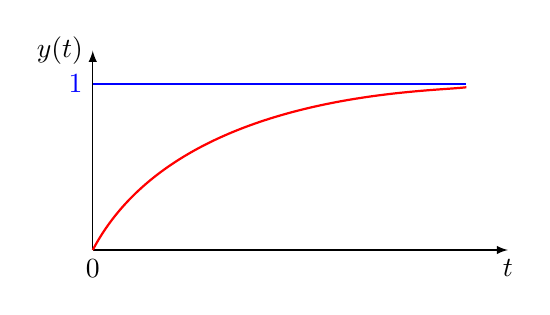
\begin{tikzpicture}[x=3em,y=6em]
\tikzstyle{arrow}=[draw,-latex]
\tikzstyle{line}=[draw,thick]
\path[arrow](0,0)--(5,0)node[below,at start]{$0$}node[below,at end,color=black]{$t$};
\path[arrow](0,0)--(0,1.2)node[left,at end]{$y(t)$};
\path[line,blue](0,1)--(4.5,1)node[left,at start]{$1$};
\path[line,red](0,0)..controls(1,0.95)and(4,0.95)..(4.5,.98);
\end{tikzpicture}\\
$\zeta>1$时，$\zeta$越大，曲线单调上升过程越缓慢；
\end{frame}

\begin{frame}{（临界阻尼，过阻尼）时系统分析}
2、临界阻尼：$\zeta=1$
\begin{description}
\item[闭环极点]$s_{1,2}=-\omega_n$
\item[闭环传函]$G_B(s)=\frac{\omega_n^2}{(s+\omega_n)^2}$
\item[单位阶跃响应]$y(t)=1-e^{-\omega_nt}(1+\omega_nt)$
\end{description}
\centering
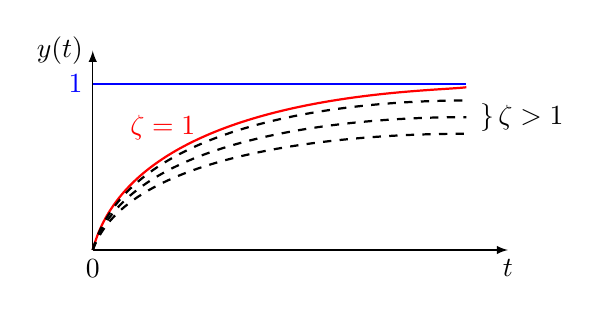
\begin{tikzpicture}[x=3em,y=6em]
\tikzstyle{arrow}=[draw,-latex]
\tikzstyle{line}=[draw,thick]
\path[arrow](0,0)--(5,0)node[below,at start]{$0$}node[below,at end,color=black]{$t$};
\path[arrow](0,0)--(0,1.2)node[left,at end]{$y(t)$};
\path[line,blue](0,1)--(4.5,1)node[left,at start]{$1$};
\path[line,red](0,0)..controls(.5,0.95)and(4,0.95)..(4.5,.98)node[above=3pt,near start]{$\zeta=1$};
\path[line,dashed](0,0)..controls(.5,0.9)and(4,0.9)..(4.5,.9);
\path[line,dashed](0,0)..controls(.5,0.8)and(4,0.8)..(4.5,.8)node[right,at end]{$\left.\right\}\zeta>1$};
\path[line,dashed](0,0)..controls(.5,0.7)and(4,0.7)..(4.5,.7);
\end{tikzpicture}\\
$\zeta=1$时，处于衰减振荡与单调变化的临界状态
\end{frame}

\begin{frame}{二阶系统单位阶跃响应$\Phi(s)=\frac{\omega_n^2}{s^2+2\zeta\omega_ns+\omega_n^2}$}
\vspace{-1em}
\begin{center}
\begin{tikzpicture}[x=2em,y=2em]
\tikzstyle{arrow}=[draw,-latex]
\tikzstyle{line}=[draw,thick]
\node at (0,0){$\zeta>1$};
\path[arrow](1.5,0)--(5,0);
\path[arrow](4.5,-1)--(4.5,1)node[right,at end]{$j$};
\node[crossc,label=above:$-\frac{1}{T_2}$] at (2.5,0){};
\node[crossc,label=above:$-\frac{1}{T_1}$] at (3.5,0){};
\node at (5,-.5){$0$};

\begin{scope}[xshift=16em]
\node at (0,0){$\zeta=1$};
\path[arrow](1.5,0)--(5,0);
\path[arrow](4.5,-1)--(4.5,1)node[right,at end]{$j$};
\node[crossc] at (3,0){};
\node[crossc] at (3.1,0){};
\node at (5,-.5){$0$}; 
\end{scope}

\begin{scope}[yshift=-10em]
\node at (0,0){$\zeta<1$};
\path[arrow](2.5,0)--(5,0);
\path[arrow](4.5,-1.2)--(4.5,1.2)node[right,at end]{$j$};
\node[crossc] at (4,.8){};
\node[crossc] at (4,-.8){};
\node at (5,-.5){$0$}; 
\end{scope}

\begin{scope}[xshift=16em,yshift=-10em]
\node at (0,0){$\zeta=0$};
\path[arrow](2.5,0)--(5,0);
\path[arrow](4.5,-1.2)--(4.5,1.2)node[right,at end]{$j$};
\node[crossc] at (4.5,.8){};
\node[crossc] at (4.5,-.8){};
\node at (5,-.5){$0$}; 
\end{scope}

\begin{scope}[yshift=-5em]
\path[arrow](0,0)--(5,0);
\path[arrow](0,0)--(0,1.3);
\path[line,dotted,gray](0,1)--(5,1);
\path[line] plot file{../figs/StepXiLargerThanOne.txt} ;
\node[red] at (2.5,0.5){过阻尼};
\end{scope}

\begin{scope}[xshift=16em,yshift=-5em]
\path[arrow](0,0)--(5,0);
\path[arrow](0,0)--(0,1.3);
\path[line,dotted,gray](0,1)--(5,1);
\path[line] plot file{../figs/StepXiEqualOne.txt} ;
\node[red] at (2.5,0.5){临界阻尼};
\end{scope}

\begin{scope}[yshift=-15em]
\path[arrow](0,0)--(5,0);
\path[arrow](0,0)--(0,1.3);
\path[line,dotted,gray](0,1)--(5,1);
\path[line] plot file{../figs/StepXiSmallerThanOne.txt} ;
\node[red] at (2.5,0.5){欠阻尼};
\end{scope}

\begin{scope}[xshift=16em,yshift=-15em]
\path[arrow](0,0)--(5,0);
\path[arrow](0,0)--(0,1.3);
\path[line,dotted,gray](0,1)--(5,1);
\path[line] plot file{../figs/StepXiZero.txt} ;
\node[red] at (2.5,0.5){零阻尼};
\end{scope}

\path[line,dashed,gray](-1,1.6)-|(13.5,-7.8)-|(-1,1.6);
\path[line,dashed,gray](6.25,-7.8)--(6.25,1.6);
\path[line,dashed,gray](-1,-3.1)--(13.5,-3.1);
\end{tikzpicture}
\end{center}
\end{frame}

\subsection{小结}
\begin{frame}{小结}
\vspace{-0.5em}
\begin{enumerate}
\item 传递函数标准形式及分类
\item $0\le\zeta<1$（欠阻尼，零阻尼）时系统 动态性能
\vspace{-1.5em}
\begin{columns}[T]
\column{.5\textwidth}
\begin{align*}
&\Phi(s)=\frac{\omega_n^2}{s^2+2\zeta\omega_ns+\omega_n^2}\quad0\le<1\\
(1)\ &0\le\zeta<1\text{时系统极点的两种表示方法}\\
(2)\ &0\le\zeta<1\text{单位阶跃响应}h(t)\text{表达式}\\
&h(t)=1-\frac{e^{-\zeta\omega_nt}}{\sqrt{1-\zeta^2}}\sin(\sqrt{1-\zeta^2}\omega_nt+\beta)\\
(3)\ &0\le\zeta<1\text{动态指标计算公式}\\
&t_p=\frac{\pi}{\sqrt{1-\zeta^2}\omega_n}\quad\sigma\%=e^{-\zeta\pi/\sqrt{1-\zeta^2}}\quad t_s=\frac{3.5}{\zeta\omega_n}\\
(4)\ &\text{“最佳阻尼比”概念}\\
(5)\ &\text{动态性能随系统极点分布变化的规律}
\end{align*}
\column{.5\textwidth}
\begin{tikzpicture}[x=1em,y=1em]
\tikzstyle{arrow}=[draw,-latex]
%\tikzstyle{dash}=[draw,thick,dashed,cyan]
\path[arrow](-5,0)--(1,0);
\path[arrow](0,-1)--(0,5)node[right,at end]{$\rj$};
\path[daline](-4,0)|-(0,4)node[below,at start]{$\sigma=-\zeta\omega_n$}node[right,at end]{$\omega_d$};
\path[daline](0,0)--(-4,4)node[above,midway]{$\omega_n$};
\node[crossc,label=left:$\lambda_1$]at(-4,4){};
\path[arrow,thick](-1.5,0)node[above left]{$\beta$}arc(180:135:1.5); 
\node[cyan] at (-2,-2.5){$\omega_d=\sqrt{1-\zeta^2}\omega_n$};
\end{tikzpicture}
\end{columns}
\item $\zeta\ge1$（临界阻尼，过阻尼）时系统分析
\end{enumerate}
\end{frame}

%:Lecture 4: 高阶系统
\lecture{高阶系统的响应}{Lecture 4}
\setcounter{section}{3}
\section{高阶系统的响应}
\begin{frame}{概要}
\begin{itemize}
\item 前面研究了两种低阶系统；
\item 用高阶微分方程描述的系统为高阶系统；
\item 工程实际中的系统绝大多数为高阶系统；
\item 高阶系统的解析解比较复杂，有时高阶系统可以用低阶系统的响应来近似——主导极点。
\end{itemize}
\end{frame}

\subsection{高阶系统的一般形式}
\begin{frame}{高阶系统的一般形式}
\begin{center}
\begin{tikzpicture}[x=2em,y=2em]
	\tikzstyle{line}=[draw=blue,-latex,thick]
	\tikzstyle{block}=[rectangle,draw,,anchor=west,thick]
	\path[line](0,0)--node[above,at start]{\color{red}$R(s)$}++(2em,0)coordinate(t);
	\node[cross,anchor=west](c)at(t){};
	\path[line](c.east)--++(1,0)coordinate(t);
	\node[block](b1)at (t){$G(s)$};
	\node[block,below of=b1](b2){$H(s)$};
	\path[line](b1.east)--++(1,0)coordinate(o)--node[above,at end]{\color{red}$Y(s)$}++(1,0);
	\path[line](o)|-(b2.east);
	\path[line](b2.west)-|(c.south)node[right,at end]{$-$};
\end{tikzpicture}
\end{center} 
\alert{闭环传函}
$$G(s)=\frac{Y(s)}{R(s)}=\frac{G(s)}{1+G(s)H(s)}=\frac{b_ms^m+b_{m-1}s^{m-1}+\cdots+b_1s+b_0}{a_ns^n+a_{n-1}s^{n-1}+\cdots+a_1s+a_0}$$
\end{frame}

\subsection{高阶系统的单位阶跃响应}
\begin{frame}{高阶系统的单位阶跃响应}
\begin{align*}
Y(s)=G(s)R(s)=&\ \frac{b_ms^m+b_{m-1}s^{m-1}+\cdots+b_1s+b_0}{a_ns^n+a_{n-1}s^{n-1}+\cdots+a_1s+a_0}\frac{1}{s}\\
=&\ \frac{K\prod_{i=1}^m(s+z_i)}{\prod_{j=1}^q(s+s_j)\prod_{k=1}^r(s^2+\zeta_k\omega_ks+\omega_k^2)}\frac{1}{s}
\end{align*}
$q$为实数极点的个数，$r$为共轭复数极点的个数，$q+2r\ge m$。设上述极点互异并都位于平面的左半平面，则经过整理后
$$Y(s)=\frac{A_0}{s}+\sum_{j=1}^q\frac{A_j}{s+s_j}+\sum_{k=1}^r\frac{B_ks+C_k}{s^2+2\zeta_k\omega_ks+\omega_k^2}$$
\end{frame}

\begin{frame}{高阶系统的单位阶跃响应}
经拉氏反变换
\begin{align*}
y(t)=&\ A_0+\sum_{j=1}^qA_je^{-s_jt}\\
&+\sum_{k=1}^r \left[ B_ke^{-\zeta_k\omega_kt}\cos\sqrt{1-\zeta_k^2}\omega_kt+C_ke^{-\zeta_k\omega_kt}\sin\sqrt{1-\zeta_k^2}\omega_kt \right]
\end{align*}
这表明：高阶系统的时间响应是由若干一阶系统和二阶系统的时间响应函数项组成的。
\end{frame}

\begin{frame}{高阶系统的近似分析}
\begin{itemize}
\item 高阶系统的相应可以通过主导极点法进行近似；
\item 高阶系统可以近似成低阶系统来分析；
\item 学习了系统的根轨迹后将详细说明为什么高阶系统可以近似来分析。
\end{itemize}
\end{frame}

\lecture{线性系统的稳定性分析}{Lecture 5}
\setcounter{section}{4}
\section{线性系统的稳定性分析}
\subsection{稳定性的概念}
\begin{frame}{稳定性的概念}
 稳定是控制系统正常工作的首要条件。分析、判定系统的稳定性，并提出确保系统稳定的条件是自动控制理论的基本任务之一。
\begin{center}
\begin{tikzpicture}[x=1em,y=1em]
\draw[pattern=north east lines,pattern color=gray](0,0)parabola bend(3,-2) (6,0)--(6,-4)--(0,-4)--(0,0);
\draw[fill=gray,thick](3,-1.5)circle(0.5);
\node at (3,-5){稳定};

\begin{scope}[xshift=7em]
\draw[pattern=north east lines,pattern color=gray](0,-2)rectangle(6,-4);
\draw[fill=gray,thick](3,-1.5)circle(0.5);
\node at (3,-5){临界稳定};
\end{scope}

\begin{scope}[xshift=14em]
\draw[pattern=north east lines,pattern color=gray](0,-4)parabola bend(3,-2) (6,-4)--(0,-4);
\draw[fill=gray,thick](3,-1.5)circle(0.5);
\node at (3,-5){不稳定};
\end{scope}
\end{tikzpicture}
 
\end{center}
\begin{block}{定义：}
	如果在扰动作用下系统偏离了原来的平衡状态，当扰动消失后，系统能够以足够的准确度恢复到原来的平衡状态，则系统是稳定的；否则，系统不稳定。
\end{block}
\end{frame}

\subsection{稳定的充要条件}
\begin{frame}{稳定的充要条件}
\vspace{-0.5em}
根据系统稳定的定义，若$\limit{t}{\infty}k(t)=0$，则系统是稳定的。  
\vspace{-0.5em}
\begin{align*}
\text{必要性}\quad&\Phi(s)=\frac{N(s)}{D(s)}=\frac{b_m(s-z_1)(s-z_2)\cdots(s-z_m)}{a_n(s-\lambda_1)(s-\lambda_2)\cdots(s-\lambda_n)}\\
&C(s)=\Phi(s)=\frac{A_1}{s-\lambda_1}+\frac{A_2}{s-\lambda_2}+\cdots+\frac{A_n}{s-\lambda_n}=\sum_{i=1}^n\frac{A_i}{s-\lambda_i}\\
&k(t)=A_1e^{\lambda_1t}+A_2e^{\lambda_2t}+\cdots+A_ne^{\lambda_nt}=\sum_{i=1}^nA_ie^{\lambda_it}\\
&\limit{t}{\infty}k(t)=\limit{t}{\infty}\sum_{i=1}^nA_ie^{\lambda_it}=0\Rightarrow\lambda_i<0\quad i=1,2,\cdots,n\\
\text{充分性}\quad&\lambda_i<0\quad i=1,2,\cdots,n\Rightarrow k(t)=\sum_{i=1}^nA_ie^{\lambda_it}\mathop{\longrightarrow}^{t\rightarrow\infty}0
\end{align*}
\alert{系统稳定的充要条件：}{\color{red}系统所有闭环特征根均具有负的实部，或所有闭环特征根均位于左半s平面。}
\end{frame}

\subsection{稳定判据：方法}
\begin{frame}{稳定判据}
$$D(s)=a_ns^n+a_{n-1}s^{n-1}+\cdots+a_1s+a_0=0\quad(a_n>0)$$
(1) 必要条件~~\tikz[baseline=-3pt]{\node[top color=green,bottom color=green,middle color=white]{$a_i>0$};}$\quad i=1,2,\cdots,n-1$
\begin{align*}
\text{说明：}D(s)=&\ (s+1)(s+2)(s+3)\\
=&\ (s^2+3s+2)(s+3)\\
=&\ s^3+6s^2+11s+6
\end{align*}
例$\begin{cases}D(s)=s^5+6s^4+9s^3-2s^2+8s+12=0&\text{\color{red}不稳定}\\D(s)=s^5+4s^4+6s^2+9s+8=0&\text{\color{red}不稳定}\\D(s)=-s^4-5s^3-7s^2-2s-10=0&\text{\color{red}可能稳定}\end{cases}$
\end{frame}

\begin{frame}{Routh-Hurwitz判据}
	\centering
	\tiny
	\begin{tikzpicture}[x=1.3em, y=1.3em]
		\onslide<1->{\node[label=below:\begin{tabular}{c}Edward John Routh\\ (1831-1907)\\ {FRS, Senior Wrangler}\\{"Let us consider}\\ {a spherical ship"}\end{tabular}] (routh) at (0,0) {\includegraphics[height=3cm]{../figs/C3Edward_J_Routh.jpg}};}
		\onslide<2->{\node[label=below:\begin{tabular}{c}Adolf Hurwitz\\(1859-1919)\end{tabular}] (hurwitz) at (0,-16) {\includegraphics[height=3cm]{../figs/C3Adolf_Hurwitz.jpg}};}
		\onslide<4->{\node[label=below:\begin{tabular}{c}James Clerk Maxwell\\ (1831-1879)\\ {FRS, FRSE, Second Wrangler}\\{Einstein: I stand on}\\ {the shoulders of Maxwell}\end{tabular}] (maxwell) at (13,0) {\includegraphics[height=3cm]{../figs/C3James_Clerk_Maxwell.png}};}
		\onslide<5->{\node[label=below:\begin{tabular}{c}Sir George Gabriel Stokes\\(1819-1903)\\{PRS, Senior Wrangler}\end{tabular}] (stokes) at (26,0) {\includegraphics[height=3cm]{../figs/C3Ggstokes.jpg}};}		
		\onslide<6->{\node[label=below:\begin{tabular}{c}Lord Kelvin\\(1824-1907)\\{PRS, FRSE, Second Wrangler}\end{tabular}] (kelvin) at (39,0) {\includegraphics[height=3cm]{../figs/C3Lord_Kelvin.jpg}};}
		\onslide<3->{\node[label=below:\begin{tabular}{c}William Hopkins\\(1793-1866)\\{FRS, Wrangler maker}\end{tabular}] (hopkins) at (26,-15) {\includegraphics[height=3cm]{../figs/C3WilliamHopkins.jpg}};}
	\end{tikzpicture}
\end{frame}

\begin{frame}{稳定判据}
(2) 劳斯（Routh）判据
$$D(s)=a_ns^n+a_{n-1}s^{n-1}+\cdots+a_1s+a_0=0\quad(a_n>0)$$
劳斯表
\vspace{-2em}
\begin{figure}
\centering
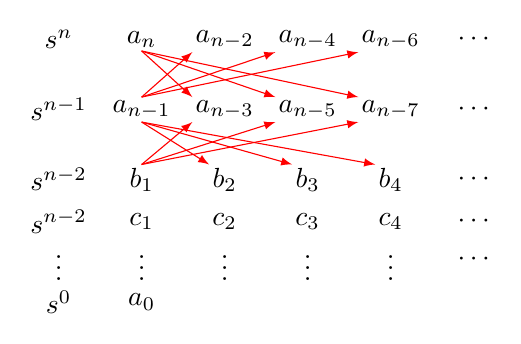
\begin{tikzpicture}[auto,node distance=3em,every node/.style={inner sep=1pt}]
\tikzstyle{arrow}=[draw,red,-latex]
\node(n00){$s^n$};
\node[right of=n00](n01){$a_n$}; 
\node[right of=n01](n02){$a_{n-2}$};
\node[right of=n02](n03){$a_{n-4}$}; 
\node[right of=n03](n04){$a_{n-6}$};
\node[right of=n04](n05){$\cdots$};

\node[below of=n00,below=-1em](n10){$s^{n-1}$};
\node[right of=n10](n11){$a_{n-1}$};
\node[right of=n11](n12){$a_{n-3}$};
\node[right of=n12](n13){$a_{n-5}$};
\node[right of=n13](n14){$a_{n-7}$};
\node[right of=n14](n15){$\cdots$};

\node[below of=n10,below=-1em](n20){$s^{n-2}$};
\node[right of=n20](n21){$b_1$};
\node[right of=n21](n22){$b_2$};
\node[right of=n22](n23){$b_3$};
\node[right of=n23](n24){$b_4$};
\node[right of=n24](n25){$\cdots$};

\node[below of=n20,below=-2em](n30){$s^{n-2}$};
\node[right of=n30](n31){$c_1$};
\node[right of=n31](n32){$c_2$};
\node[right of=n32](n33){$c_3$};
\node[right of=n33](n34){$c_4$};
\node[right of=n34](n35){$\cdots$};

\node[below of=n30,below=-2.5em](n40){$\vdots$};
\node[right of=n40](n41){$\vdots$};
\node[right of=n41](n42){$\vdots$};
\node[right of=n42](n43){$\vdots$};
\node[right of=n43](n44){$\vdots$};
\node[right of=n44](n45){$\cdots$};

\node[below of=n40,below=-2em](n50){$s^0$};
\node[right of=n50](n51){$a_0$};

\path[arrow](n01.south)--(n12.north west);
\path[arrow](n01.south)--(n13.north west);
\path[arrow](n01.south)--(n14.north west);

\path[arrow](n11.north)--(n02.south west);
\path[arrow](n11.north)--(n03.south west);
\path[arrow](n11.north)--(n04.south west);

\path[arrow](n11.south)--(n22.north west);
\path[arrow](n11.south)--(n23.north west);
\path[arrow](n11.south)--(n24.north west);

\path[arrow](n21.north)--(n12.south west);
\path[arrow](n21.north)--(n13.south west);
\path[arrow](n21.north)--(n14.south west);
\end{tikzpicture}
\end{figure} 
劳斯表第一列元素均大于零时系统稳定，否则系统不稳定    
且第一列元素符号改变的次数就是特征方程中正实部根的个数 
\end{frame}

\subsection{稳定判据：实例}
\begin{frame}{\example{稳定判据A}{ex:routh1}}
\vspace{-1em}
$$D(s)=s^4+5s^3+7s^2+2s+10=0$$ 
\textsf{解：}列劳斯表
\begin{figure}
\centering
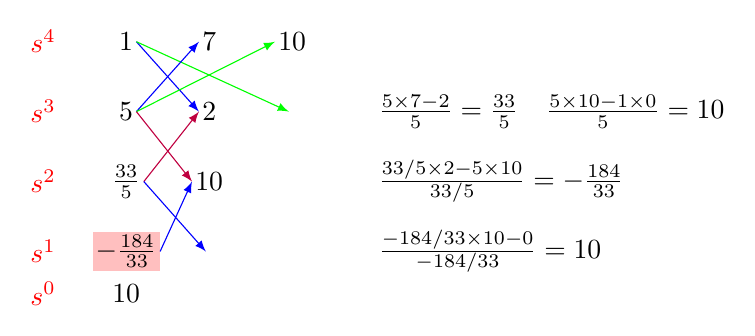
\begin{tikzpicture}[auto,node distance=3em,every node/.style={inner sep=1pt}]
\tikzstyle{arrow}=[draw,-latex]
\node[red](n00){$s^4$};
\node[right of=n00](n01){$1$}; 
\node[right of=n01](n02){$7$};
\node[right of=n02](n03){$10$}; 

\node[below of=n00,below=-1em,red](n10){$s^3$};
\node[right of=n10](n11){$5$};
\node[right of=n11](n12){$2$};
\node[right of=n12](n13){};

\node[below of=n10,below=-1em,red](n20){$s^2$};
\node[right of=n20](n21){$\frac{33}{5}$};
\node[right of=n21](n22){$10$};
\node[right of=n22](n23){};

\node[below of=n20,below=-1em,red](n30){$s^1$};
\node[right of=n30,fill=pink](n31){$-\frac{184}{33}$};
\node[right of=n31](n32){};
\node[right of=n32](n33){};

\node[below of=n30,below=-2em,red](n40){$s^0$};
\node[right of=n40](n41){$10$};

\path[arrow,blue](n01.east)--(n12.west);
\path[arrow,green](n01.east)--(n13.west);

\path[arrow,blue](n11.east)--(n02.west);
\path[arrow,green](n11.east)--(n03.west);

\path[arrow,purple](n11.east)--(n22.west);
\path[arrow,purple](n21.east)--(n12.west);
\path[arrow,blue](n21.east)--(n32.west);
\path[arrow,blue](n31.east)--(n22.west);

\node[right of=n13,anchor=west]{$\frac{5\times7-2}{5}=\frac{33}{5}\quad\frac{5\times10-1\times0}{5}=10$};
\node[right of=n23,anchor=west]{$\frac{33/5\times2-5\times10}{33/5}=-\frac{184}{33}$};
\node[right of=n33,anchor=west]{$\frac{-184/33\times10-0}{-184/33}=10$};
\end{tikzpicture}
\end{figure}  
劳斯表第一列元素变号 2次，有2个正根，系统{\color{red}不稳定}。 
\end{frame}

\begin{frame}{\example{稳定判据B}{ex:routh2}}
(3) 劳斯判据特殊情况处理
$D(s)=s^3-3s+2=0$，判定在右半平面的极点数。\\
\textsf{解：}列劳斯表
\begin{figure}
\centering
\begin{tikzpicture}[x=1em,y=1em,node distance=3em,every node/.style={inner sep=1pt}]
\tikzstyle{arrow}=[draw,-latex]
\node[red](n00){$s^3$};
\node[right of=n00](n01){$1$}; 
\node[right of=n01](n02){$-3$};

\node[below of=n00,below=-1em,red](n10){$s^2$};
\node[right of=n10](n11){$\epsilon$};
\node[right of=n11](n12){$2$};

\node[below of=n10,below=-1em,red](n20){$s^1$};
\node[right of=n20,fill=pink](n21){$-\infty$};
\node[right of=n21](n22){$0$};

\node[below of=n20,below=-1em,red](n30){$s^0$};
\node[right of=n30](n31){$2$};
\node[right of=n31](n32){};

\path[arrow,blue](n01.east)--(n12.west);
\path[arrow,blue](n11.east)--(n02.west);

\path[arrow,purple](n11.east)--(n22.west);
\path[arrow,purple](n21.east)--(n12.west);

\path[draw,green](-1,-4)--(7,-4);
\path[draw,green](1.5,0)--(1.5,-8);
\node[right of=n12,anchor=west]{$\frac{-3\epsilon-2}{\epsilon}=-\infty$};
\node[right of=n22,anchor=west]{$\frac{-2\times\infty-0}{-\infty}=2$};
\node[right of=n12,anchor=west,right=8em,text width=11em,red]{某行第一列元素为$0$，而该行元素不全为$0$时：将此$0$改为$\epsilon$ ，继续运算。};
\end{tikzpicture}
\end{figure}  
劳斯表第一列元素变号 2次，有2个正根，系统{\color{red}不稳定}。 
\end{frame}

\begin{frame}{\example{稳定判据C}{ex:routh3}}
\vspace{-1em}
$$D(s)=s^5+3s^4+12s^3+20s^2+35s+25=0$$ 
\textsf{解：}列劳斯表
\vspace{-.5em}
\begin{columns}[T]
\column{.5\textwidth}
\begin{figure}
\centering
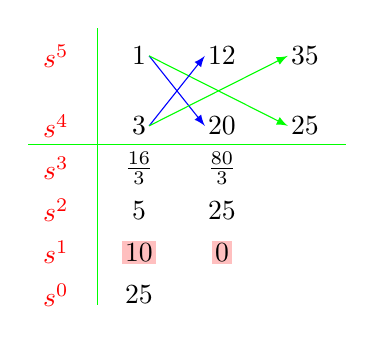
\begin{tikzpicture}[x=1em,y=1em,node distance=3em,every node/.style={inner sep=1pt}]
\tikzstyle{arrow}=[draw,-latex]
\node[red](n00){$s^5$};
\node[right of=n00](n01){$1$}; 
\node[right of=n01](n02){$12$};
\node[right of=n02](n03){$35$}; 

\node[below of=n00,below=-1em,red](n10){$s^4$};
\node[right of=n10](n11){$3$};
\node[right of=n11](n12){$20$};
\node[right of=n12](n13){$25$};

\node[below of=n10,below=-2em,red](n20){$s^3$};
\node[right of=n20](n21){$\frac{16}{3}$};
\node[right of=n21](n22){$\frac{80}{3}$};

\node[below of=n20,below=-2em,red](n30){$s^2$};
\node[right of=n30](n31){$5$};
\node[right of=n31](n32){$25$};

\node[below of=n30,below=-2em,red](n40){$s^1$};
\node[right of=n40,fill=pink](n41){$10$};
\node[right of=n41,fill=pink](n42){$0$};

\node[below of=n40,below=-2em,red](n50){$s^0$};
\node[right of=n50](n51){$25$};

\path[arrow,blue](n01.east)--(n12.west);
\path[arrow,green](n01.east)--(n13.west);

\path[arrow,blue](n11.east)--(n02.west);
\path[arrow,green](n11.east)--(n03.west);

\path[draw,green](-1,-3.2)--(10.5,-3.2);
\path[draw,green](1.5,1)--(1.5,-9);
\end{tikzpicture}
\end{figure}  
\column{.5\textwidth}
{\color{blue}出现全零行时：}\\
用上一行元素组成辅助方程，将其对$s$求导一次，
用新方程的系数代替全零行系数，之后继续运算。\\
列辅助方程：$5s^2+25=0$
$$\dod{}{s}(5s^2+25)=10s+0$$
\end{columns}
\vspace{.5em}
出现全零行时，系统可能出现一对共轭虚根；或一对符号
相反的实根；或两对实部符号相异、虚部相同的复根。       
\end{frame}

\begin{frame}{\example{稳定判据D}{ex:routh4}}
\vspace{-1em}
$$D(s)=s^5+2s^4-s-2=0\onslide<8->{{\color{red}\ =(s+2)(s+1)(s-1)(s+j)(s-j)}}$$ 
解：列劳斯表
\vspace{-.5em}
\begin{columns}[T]
\column{.5\textwidth}
\begin{figure}
\centering
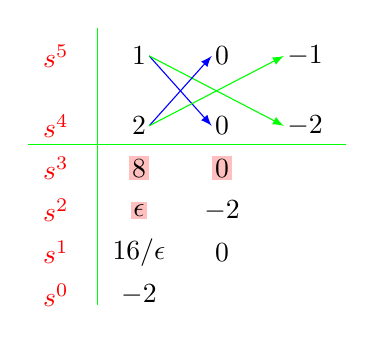
\begin{tikzpicture}[x=1em,y=1em,node distance=3em,every node/.style={inner sep=1pt}]
\tikzstyle{arrow}=[draw,-latex]
\onslide<2->{\node[red](n00){$s^5$};}
\onslide<3->{\node[right of=n00](n01){$1$}; 
\node[right of=n01](n02){$0$};
\node[right of=n02](n03){$-1$}; }

\onslide<2->{\node[below of=n00,below=-1em,red](n10){$s^4$};}
\onslide<3->{\node[right of=n10](n11){$2$};
\node[right of=n11](n12){$0$};
\node[right of=n12](n13){$-2$};}

\onslide<2->{\node[below of=n10,below=-2em,red](n20){$s^3$};}
\onslide<4->{\node[right of=n20,fill=pink](n21){$8$};
\node[right of=n21,fill=pink](n22){$0$};}

\onslide<2->{\node[below of=n20,below=-2em,red](n30){$s^2$};}
\onslide<5->{\node[right of=n30,fill=pink](n31){$\epsilon$};
\node[right of=n31](n32){$-2$};}

\onslide<2->{\node[below of=n30,below=-2em,red](n40){$s^1$};}
\onslide<6->{\node[right of=n40](n41){$16/\epsilon$};
\node[right of=n41](n42){$0$};}

\onslide<2->{\node[below of=n40,below=-2em,red](n50){$s^0$};}
\onslide<7->{\node[right of=n50](n51){$-2$};}

\onslide<3->{\path[arrow,blue](n01.east)--(n12.west);
\path[arrow,green](n01.east)--(n13.west);

\path[arrow,blue](n11.east)--(n02.west);
\path[arrow,green](n11.east)--(n03.west);
\path[draw,green](-1,-3.2)--(10.5,-3.2);
\path[draw,green](1.5,1)--(1.5,-9);}
\end{tikzpicture}
\end{figure}  
\column{.5\textwidth}
\onslide<4->{{\color{blue}列辅助方程：}\\
$$2s^4-2=0$$
$$\dod{}{s}(2s^4-2)=8s^3=0$$}
\end{columns}
\vspace{.5em}
\onslide<8->{第一列元素变号一次，有一个正根，系统不稳定}
\end{frame}

\begin{frame}{\example{稳定判据E}{ex:routh5}}
\vspace{-1em}
\begin{columns}[T]
	\column{.6\textwidth}
	系统结构图如下，
	\begin{enumerate}
		\item 确定使系统稳定的参数$(K,\zeta)$的范围;
		\item 当$\zeta=2$时，确定使全部极点均位于$s=-1$之左的$K$值范围。
	\end{enumerate}
	\column{.4\textwidth}
	\scalebox{0.8}{
	\begin{tikzpicture}[x=1em,y=1em]
		\tikzstyle{line}=[draw=blue,-latex,thick]
		\tikzstyle{block}=[rectangle,draw,,anchor=west,thick]
		\path[line](0,0)--node[above,at start]{\color{red}$R(s)$}++(2em,0)coordinate(t);
		\node[cross,anchor=west](c)at(t){};
		\path[line](c.east)--++(1,0)coordinate(t);
		\node[block](b)at(t){$\frac{K_a}{s(s^2+20\zeta s+100)}$};
		\path[line](b.east)--++(1,0)coordinate(o)--node[above,at end]{\color{red}$C(s)$}++(1,0);
		\path[line](o)--++(0,-2)-|node[right,at end]{$-$}(c.south);
		\end{tikzpicture}}
	\end{columns}
\begin{align*}
\textsf{解：}(1)\ &G(s)=\frac{K_a}{s(s^2+20\zeta s+100)}\quad K=\frac{K_a}{100}\\
&D(s)=s^3+20\zeta s^2+100s+100K=0
\end{align*}

\begin{figure}
\centering
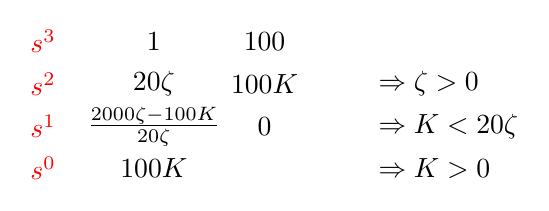
\begin{tikzpicture}[x=1em,y=1em,node distance=4em,every node/.style={inner sep=1pt}]
\tikzstyle{arrow}=[draw,-latex]
\node[red](n00){$s^3$};
\node[right of=n00](n01){$1$}; 
\node[right of=n01](n02){$100$};

\node[below of=n00,below=-3em,red](n10){$s^2$};
\node[right of=n10](n11){$20\zeta$};
\node[right of=n11](n12){$100K$};
\node[right of=n12,anchor=west](n13){$\Rightarrow\zeta>0$};

\node[below of=n10,below=-3em,red](n20){$s^1$};
\node[right of=n20](n21){$\frac{2000\zeta-100K}{20\zeta}$};
\node[right of=n21](n22){$0$};
\node[right of=n22,anchor=west](n23){$\Rightarrow K<20\zeta$};

\node[below of=n20,below=-3em,red](n30){$s^0$};
\node[right of=n30](n31){$100K$};
\node[right of=n31](n32){};
\node[right of=n32,anchor=west](n33){$\Rightarrow K>0$};
\end{tikzpicture}
\end{figure}
\end{frame}

\addtocounter{example}{-1}
\begin{frame}{\example{稳定判据E}{}}
(2)当\,$\zeta=2$ 时，确定使全部极点均位于$s=-1$之左的$K$值范围。
 
当\,$\zeta=2$ 时，进行平移变换：$s=\hat{s}-1$
\begin{align*}
D(s)=&\ s^3+20\times2s^2+100s+100K=0\\
\downarrow&\ s=\hat{s}-1\\
D(\hat{s})=&\ (\hat{s}-1)^3+40(\hat{s}-1)^2+100(\hat{s}-1)+100K=0\\
=&\ \hat{s}^3+37\hat{s}^2+23\hat{s}+(100K-61)=0
\end{align*}
\begin{figure}
\centering
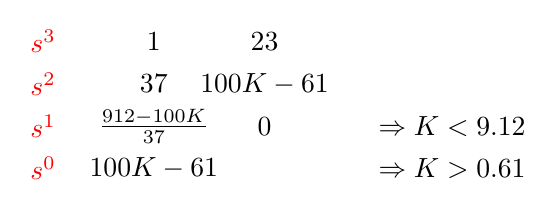
\begin{tikzpicture}[x=1em,y=1em,node distance=4em,every node/.style={inner sep=1pt}]
\tikzstyle{arrow}=[draw,-latex]
\node[red](n00){$s^3$};
\node[right of=n00](n01){$1$}; 
\node[right of=n01](n02){$23$};

\node[below of=n00,below=-3em,red](n10){$s^2$};
\node[right of=n10](n11){$37$};
\node[right of=n11](n12){$100K-61$};

\node[below of=n10,below=-3em,red](n20){$s^1$};
\node[right of=n20](n21){$\frac{912-100K}{37}$};
\node[right of=n21](n22){$0$};
\node[right of=n22,anchor=west](n23){$\Rightarrow K<9.12$};

\node[below of=n20,below=-3em,red](n30){$s^0$};
\node[right of=n30](n31){$100K-61$};
\node[right of=n31](n32){};
\node[right of=n32,anchor=west](n33){$\Rightarrow K>0.61$};
\end{tikzpicture}
\end{figure}
\end{frame}

\subsection{课程小结}
\begin{frame}{课程小结}
\begin{description}
\item[\S3.5.1]\alert{稳定性的概念} \tikz[baseline=-4pt]{\node[fill=green!50!white]{$\limit{t}{\infty}k(t)=0$};}
\item[\S3.5.2]\alert{稳定的充要条件} \\ 系统闭环特征方程的所有根都具有负的实部\\
或所有闭环特征根均位于左半$s$平面 
\item[\S3.5.3]\alert{稳定判据}
$$D(s)=a_ns^n+a_{n-1}s^{n-1}+\cdots+a_1s+a_0=0$$
\vspace{-1em}
\begin{enumerate}
\item 判定稳定的必要条件\tikz[baseline=-4pt]{\node[fill=green!50!white]{$a_i>0$};}
\item 劳斯判据
\item 劳斯判据特殊情况的处理
\item 劳斯判据的应用（判定稳定性，确定稳定的参数范围） 
\end{enumerate}
\end{description}
\end{frame}

%:Lecture 6: 稳态误差
\lecture{稳态误差}{Lecture 6}
\section*{课程回顾}
\begin{frame}{课程回顾}
\begin{description}
\item[\S3.5.1]\alert{稳定性的概念} \tikz[baseline=-4pt]{\node[fill=green!50!white]{$\limit{t}{\infty}k(t)=0$};}
\item[\S3.5.2]\alert{稳定的充要条件} \\ 系统闭环特征方程的所有根都具有负的实部\\
或所有闭环特征根均位于左半$s$平面 
\item[\S3.5.3]\alert{稳定判据}
$$D(s)=a_ns^n+a_{n-1}s^{n-1}+\cdots+a_1s+a_0=0$$
\vspace{-1em}
\begin{enumerate}
\item 判定稳定的必要条件\tikz[baseline=-4pt]{\node[fill=green!50!white]{$a_i>0$};}
\item 劳斯判据
\item 劳斯判据特殊情况的处理
\item 劳斯判据的应用（判定稳定性，确定稳定的参数范围） 
\end{enumerate}
\end{description}
\end{frame}

\begin{frame}{劳斯（Routh）判据} 
$$D(s)=a_ns^n+a_{n-1}s^{n-1}+\cdots+a_1s+a_0=0\quad(a_n>0)$$
劳斯表
\vspace{-2em}
\begin{figure}
\centering
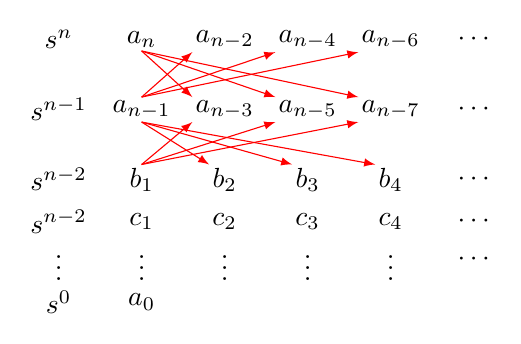
\begin{tikzpicture}[auto,node distance=3em,every node/.style={inner sep=1pt}]
\tikzstyle{arrow}=[draw,red,-latex]
\node(n00){$s^n$};
\node[right of=n00](n01){$a_n$}; 
\node[right of=n01](n02){$a_{n-2}$};
\node[right of=n02](n03){$a_{n-4}$}; 
\node[right of=n03](n04){$a_{n-6}$};
\node[right of=n04](n05){$\cdots$};

\node[below of=n00,below=-1em](n10){$s^{n-1}$};
\node[right of=n10](n11){$a_{n-1}$};
\node[right of=n11](n12){$a_{n-3}$};
\node[right of=n12](n13){$a_{n-5}$};
\node[right of=n13](n14){$a_{n-7}$};
\node[right of=n14](n15){$\cdots$};

\node[below of=n10,below=-1em](n20){$s^{n-2}$};
\node[right of=n20](n21){$b_1$};
\node[right of=n21](n22){$b_2$};
\node[right of=n22](n23){$b_3$};
\node[right of=n23](n24){$b_4$};
\node[right of=n24](n25){$\cdots$};

\node[below of=n20,below=-2em](n30){$s^{n-2}$};
\node[right of=n30](n31){$c_1$};
\node[right of=n31](n32){$c_2$};
\node[right of=n32](n33){$c_3$};
\node[right of=n33](n34){$c_4$};
\node[right of=n34](n35){$\cdots$};

\node[below of=n30,below=-2.5em](n40){$\vdots$};
\node[right of=n40](n41){$\vdots$};
\node[right of=n41](n42){$\vdots$};
\node[right of=n42](n43){$\vdots$};
\node[right of=n43](n44){$\vdots$};
\node[right of=n44](n45){$\cdots$};

\node[below of=n40,below=-2em](n50){$s^0$};
\node[right of=n50](n51){$a_0$};

\path[arrow](n01.south)--(n12.north west);
\path[arrow](n01.south)--(n13.north west);
\path[arrow](n01.south)--(n14.north west);

\path[arrow](n11.north)--(n02.south west);
\path[arrow](n11.north)--(n03.south west);
\path[arrow](n11.north)--(n04.south west);

\path[arrow](n11.south)--(n22.north west);
\path[arrow](n11.south)--(n23.north west);
\path[arrow](n11.south)--(n24.north west);

\path[arrow](n21.north)--(n12.south west);
\path[arrow](n21.north)--(n13.south west);
\path[arrow](n21.north)--(n14.south west);
\end{tikzpicture}
\end{figure} 
劳斯表第一列元素均大于零时系统稳定，否则系统不稳定    
且第一列元素符号改变的次数就是特征方程中正实部根的个数 
\end{frame}

\setcounter{section}{5}
\section{线性系统的稳态误差}
\begin{frame}{概述}
\begin{itemize}
\item 稳态误差是系统的稳态性能指标，
是对系统控制精度的度量。
\item 对稳定的系统研究稳态误差才有意义，
所以计算稳态误差应以系统稳定为前提。 
\item 本讲只讨论系统的原理性误差，即结构、数和输入信号引起的误差，不考虑由于非线性因素引起的误差。
\item 通常把在阶跃输入作用下没有原理性稳态误差的系统称为无差系统；而把有原理性稳态误差的系统称为有差系统。
\end{itemize}
\end{frame}

\subsection{误差与稳态误差}
\begin{frame}{误差与稳态误差}
\begin{center}
\begin{tikzpicture}[x=2em,y=2em]
	\tikzstyle{line}=[draw=blue,-latex,thick]
	\tikzstyle{block}=[rectangle,draw,,anchor=west,thick]
	\path[line](0,0)--node[above,at start]{\color{red}$R(s)$}++(1,0)coordinate(t);
	\node[cross,anchor=west](c)at(t){};
	\path[line](c.east)--node[above]{\color{red}$E(s)$}++(1,0)coordinate(t);
	\node[block](b1)at (t){$G(s)$};
	\node[block,below of=b1](b2){$H(s)$};
	\path[line](b1.east)--++(1,0)coordinate(o)--node[above,at end]{\color{red}$C(s)$}++(1,0);
	\path[line](o)|-(b2.east);
	\path[line](b2.west)-|(c.south)node[right,at end]{$-$};
\end{tikzpicture}\\
按输入端定义的误差：\alert{$E(s)=R(s)-H(s)C(s)$}
%\vspace{1em}\\
%\begin{tikzpicture}[x=2em,y=2em]
%	\tikzstyle{line}=[draw=blue,-latex,thick]
%	\tikzstyle{block}=[rectangle,draw,,anchor=west,thick]
%	\path[line](0,0)--node[above,at start]{\color{red}$R(s)$}++(1,0)coordinate(t);
%	\node[block](b1)at (t){$\frac{1}{H(s)}$};
%	\path[line](b1.east)--node[above]{\color{red}$R'(s)$}++(1.5,0)coordinate(t);
%	\node[cross,anchor=west](c)at(t){};
%	\path[line](c.east)--node[above]{$\color{red}E'(s)$}++(1.5,0)coordinate(t);
%	\node[block](b2)at (t){$H(s)$};
%	\path[line](b2.east)--node[above]{\color{red}$E(s)$}++(1.5,0)coordinate(t);
%	\node[block](b3)at (t){$G(s)$};
%	\path[line](b3.east)--++(1,0)coordinate(o)--node[above,at end]{\color{red}$C(s)$}++(1,0);
%	\path[line](o)--++(0,-1)-|(c.south)node[right,at end]{$-$};
%\end{tikzpicture}\\
%按输出端定义的误差：\alert{$E'(s)=\frac{R(s)}{H(s)}-C(s)$}\\
\vspace{1em}\\
稳态误差： 误差中的稳态分量$e_{ss}=\lim\limits_{t\rightarrow\infty}e(t)=e(\infty)$
\end{center}
\end{frame}
 
\subsection{计算稳态误差的一般方法}
\begin{frame}{计算稳态误差的一般方法}
\begin{enumerate}
\item 判定系统的稳定性
\item 求误差传递函数
$$\Phi_e(s)=\frac{E(s)}{R(s)}, \quad \Phi_{en}(s)=\frac{E(s)}{N(s)}$$
\item 用终值定理求稳态误差
$$e_{ss}=\lim_{s\rightarrow0}s[\Phi_e(s)R(s)+\Phi_{en}(s)N(s)]$$ 
\end{enumerate}
\end{frame}

\subsection{计算稳态误差的一般方法：实例}
\begin{frame}{\example{稳态误差：终值定理A}{ex:findEss1}}
\vspace{-.5em}
下图是一个速度调节系统。确定该系统对于单位阶跃响应的稳态误差。
\begin{center}
\begin{tikzpicture}[x=2em,y=2em]
	\tikzstyle{line}=[draw=blue,-latex,thick]
	\tikzstyle{block}=[rectangle,draw,,anchor=west,thick]
	\path[line](0,0)--node[above,at start]{\color{red}$R(s)$}node[below,at start]{参考电压}++(1,0)coordinate(t);
	\node[cross,anchor=west](c)at(t){};
	\path[line](c.east)--++(1,0)coordinate(t);
	\node[block](b1)at (t){$\frac{K_1}{0.07s+1}$};
	\path[line](b1.east)--++(1,0)coordinate(t);
	\node[block](b2)at(t){$\frac{K_2}{0.24s+1}$};
	\path[line](b2.east)--++(1,0)coordinate(o)--node[above,at end]{\color{red}$C(s)$}node[below,at end]{角速度}++(1,0);
	\node[block,below of=b1](b3){$\alpha$};
	\node[block,below of=b2](b4){$K_t$};
	\path[line](o)|-(b4.east);
	\path[line](b4.west)|-(b3.east);
	\path[line](b3.west)-|(c.south)node[right,at end]{$-$};
	\node[below of=b2,below=1em]{测速机};
\end{tikzpicture}
\end{center}
\vspace{-1em}
解：误差传递函数为
$$\Phi_e(s)=\frac{1}{1+\frac{K_1}{0.07s+1}\cdot\frac{K_2}{0.24s+1}\cdot\alpha K_t}=\frac{(0.07s+1)(0.24s+1)}{(0.07s+1)(0.24s+1)+\alpha K_1K_2K_t}$$
根据劳斯判据，$1+\alpha K_1K_2K_t>0$时这个二阶系统必定稳定，根据终值定理可有
\begin{align*}
e_{ss} &=\limit{s}{0}s\Phi_e(s)R(s)=\limit{s}{0}s\frac{(0.07s+1)(0.24s+1)}{(0.07s+1)(0.24s+1)+\alpha K_1K_2K_t}\cdot\frac{1}{s}\\
&=\frac{1}{1+\alpha K_1K_2K_t}
\end{align*}
\end{frame}
 
\begin{frame}{\example{稳态误差：终值定理B}{ex:findEss2}}
\vspace{-1em}
误差定义为$E(s)=R(s)-C(s)$。(1)确定以$K_1$和$k$表示的对于单位阶跃响应输入的稳态误差。(2)选择使稳态误差为零时的$K_1$。
\vspace{-1em}
\begin{center}
\begin{tikzpicture}[x=2em,y=2em]
	\tikzstyle{line}=[draw=blue,-latex,thick]
	\tikzstyle{block}=[rectangle,draw,,anchor=west,thick]
	\path[line](0,0)--node[above,at start]{\color{red}$R(s)$}++(1,0)coordinate(t);
	\node[block](b1)at (t){$K_1$};
	\path[line](b1.east)--++(1,0)coordinate(t);
	\node[cross,anchor=west](c)at(t){};
	\path[line](c.east)--++(1,0)coordinate(t);
	\node[block](b2)at (t){$\frac{k}{(s+10)(s+12)}$};
	\path[line](b2.east)--++(1,0)coordinate(o)--node[above,at end]{\color{red}$C(s)$}++(1,0);
	\path[line](o)--++(0,-1)-|(c.south)node[right,at end]{$-$};
\end{tikzpicture} 
\end{center}
解：(1)系统总的传递函数为$\Phi(s)=\frac{K_1k}{(s+10)(s+12)+k}$
按定义，系统误差为
\begin{align*}
E(s)=&\,R(s)-C(s)=R(s)-\Phi(s)R(s)=[1-\Phi(s)]R(s)\\
=&\,\frac{(s+10)(s+12)+k-K_1k}{(s+10)(s+12)+k}\cdot\frac{1}{s}
\end{align*}
由于系统总是稳定的，
由终值定理可有\\
$
e_{ss}=\limit{s}{0}sE(s)=\limit{s}{0}s\cdot\frac{(s+10)(s+12)+k-K_1k}{(s+10)(s+12)+k}\cdot\frac{1}{s}=\frac{120+k-K_1k}{120+k}
$
(2)令$e_{ss}=0$得到$\frac{120+k-K_1k}{120+k}=0$。即稳态误差为零时有$K_1=\frac{120+k}{k}=1+\frac{120}{k}$
\end{frame}

\begin{frame}{\example{稳态误差：终值定理C}{ex:findEss3}}
\vspace{-1em}
\begin{columns}[T]
\column{.5\textwidth}
系统如右图，已知$r(t)=At^2/2$，$n(t)=At$。求系统的稳态误差。\\
解：
\column{.5\textwidth}
\vspace{-1em}
\begin{center}
\begin{tikzpicture}[x=1em,y=2em]
	\tikzstyle{line}=[draw=blue,-latex,thick]
	\tikzstyle{block}=[rectangle,draw,,anchor=west,thick]
	\path[line](0,0)--node[above,at start]{\color{red}$r$}++(1,0)coordinate(t);
	\node[cross,anchor=west](c1)at(t){};
	\path[line](c1.east)--node[above]{\color{red}$e$}++(1,0)coordinate(t);
	\node[block](b1)at (t){$\frac{K_1}{s}$};
	\path[line](b1.east)--++(1,0)coordinate(t);
	\node[cross,anchor=west](c2)at(t){};
	\path[line](c2.east)--++(1,0)coordinate(t);
	\node[block](b2)at (t){$\frac{K_2}{s}$};
	\path[line](b2.east)--++(1,0)coordinate(o)--node[above,at end]{\color{red}$c$}++(1,0);
	\node[block,below of=c2](b3){$K_3(Ts+1)$};
	\path[line](o)|-(b3.east);
	\path[line](b3.west)-|(c1.south)node[right,at end]{$-$};
	\path[line]($(c2.north)+(0,.5)$)--node[right,at start]{$\color{red}n$}(c2.north);
\end{tikzpicture} 
\end{center}
\end{columns} 
\vspace{-3em}
\begin{align*}
&G(s)=\frac{K_1K_2K_3(Ts+1)}{s^2}\quad\begin{cases}K=K_1K_2K_3\\v=2\end{cases}\\
&\Phi_e(s)=\frac{E(s)}{R(s)}=\frac{s^2}{s^2+K_1K_2K_3(Ts+1)}\\
&D(s)=s^2+K_1K_2K_3Ts+K_1K_2K_3\quad K_1K_2K_3>0\quad T>0\\
&e_{ssr}=\limit{s}{0}s\Phi_e(s)\frac{A}{s^3}=\limit{s}{0}\frac{A}{s^2}\frac{s^2}{s^2+K_1K_2K_3Ts+K_1K_2K_3}=\frac{A}{K_1K_2K_3}\\
&\Phi_{en}(s)=\frac{-K_2K_3(Ts+1)/s}{1+K_1K_2K_3(Ts+1)/s^2}=\frac{-K_2K_3s(Ts+1)}{s^2+K_1K_2K_3Ts+K_1K_2K_3}\\
&e_{ssn}=\limit{s}{0}s\Phi_{en}(s)N(s)=\limit{s}{0}s\frac{A}{s^2}\frac{-K_2K_3s(Ts+1)}{s^2+K_1K_2K_3Ts+K_1K_2K_3}=\frac{-A}{K_1}
\end{align*}
\end{frame}
 
\subsection{静态误差系数法}
\begin{frame}{静态误差系数法\,---\,$r(t)$作用时$e_{ss}$的计算规律}
$$G(s)=G_1(s)H(s)=\frac{K(\tau_1s+1)\cdots(\tau_ms+1)}{s^v(T_1s+1)\cdots(T_{n-v}s+1)}=\frac{K}{s^v}G_0(s)$$
其中$\color{red}K\text{：开环增益}\quad v\text{：型别（类型）}$
$$G_0(s)=\frac{(\tau_1s+1)\cdots(\tau_ms+1)}{(T_1s+1)\cdots(T_{n-v}s+1)}\quad\limit{s}{0}G_0(s)=1$$
\vspace{-1em}
\begin{columns}[T]
\column{.65\textwidth}
$$\Phi_e(s)=\frac{E(s)}{R(s)}=\frac{1}{1+G_1(s)H(s)}=\frac{1}{1+\frac{K}{s^v}G_0(s)}$$
$$e_{ss}=\limit{s}{0}s\Phi_e(s)R(s)=\limit{s}{0}s\cdot R(s)\cdot\frac{1}{1+\frac{K}{s^v}G_0(s)}$$
$$\text{稳态误差}\color{red}e_{ss}\color{black}\text{与}\color{red}\begin{cases}\text{输入}r(t)\text{的形式}\\\text{系统结构参数}(K,v)\end{cases}\color{black}\text{有关}$$
\column{.35\textwidth}
\vspace{-1em}
\begin{center}
\begin{tikzpicture}[x=1em,y=2em]
	\tikzstyle{line}=[draw=blue,-latex,thick]
	\tikzstyle{block}=[rectangle,draw,,anchor=west,thick]
	\path[line](0,0)--node[above,at start]{\color{red}$R(s)$}++(1,0)coordinate(t);
	\node[cross,anchor=west](c)at(t){};
	\path[line](c.east)--node[above]{\color{red}$E(s)$}++(1.8,0)coordinate(t);
	\node[block](b1)at (t){$G_1(s)$};
	\node[block,below of=b1](b2){$H(s)$};
	\path[line](b1.east)--++(1,0)coordinate(o)--node[above]{\color{red}$C(s)$}++(1,0);
	\path[line](o)|-(b2.east);
	\path[line](b2.west)-|(c.south)node[right,at end]{$-$};
\end{tikzpicture} 
\end{center}
\end{columns} 
\end{frame}

\begin{frame}{静态误差系数法\,---\,$r(t)$作用时$e_{ss}$的计算规律}
\begin{table}
\scalebox{1}{
\begin{tabular}{l}
$e_{ss}=\limit{s}{0}s\Phi_e(s)R(s)=\limit{s}{0}sR(s)\frac{1}{1+G_1(s)H(s)}=\limit{s}{0}sR(s)\frac{1}{1+\frac{K}{s^v}G_0(s)}$\vspace{1em}\\
$e_{ssp}=\limit{s}{0}s\Phi_e(s)R(s)=\limit{s}{0}s\frac{A}{s}\frac{1}{1+G_1(s)H(s)}=\frac{A}{1+\limit{s}{0}G_1(s)H(s)}=$\tikz[baseline=-2pt]{\node[fill=green!50!white]{$\frac{A}{1+K_p}$};}\\
$r(t)=A\cdot1(t)\quad\text{\alert{静态位置误差系数}}K_p=\limit{s}{0}G_1(s)H(s)=\limit{s}{0}\frac{K}{s^v}$\vspace{1em}\\
$e_{ssv}=\limit{s}{0}s\Phi_e(s)R(s)=\limit{s}{0}s\frac{A}{s^2}\frac{1}{1+G_1(s)H(s)}=\frac{A}{\limit{s}{0}sG_1(s)H(s)}=$\tikz[baseline=-2pt]{\node[fill=green!50!white]{$\frac{A}{K_v}$};}\\
$r(t)=A\cdot t\quad\text{\alert{静态速度误差系数}}K_v=\limit{s}{0}sG_1(s)H(s)=\limit{s}{0}\frac{K}{s^{v-1}}$\vspace{1em}\\
$e_{ssa}=\limit{s}{0}s\Phi_e(s)R(s)=\limit{s}{0}s\frac{A}{s^3}\frac{1}{1+G_1(s)H(s)}=\frac{A}{\limit{s}{0}s^2G_1(s)H(s)}=$\tikz[baseline=-3pt]{\node[fill=green!50!white]{$\frac{A}{K_a}$};}\\
$r(t)=\frac{A}{2}t^2\quad\text{\alert{静态加速度误差系数}}K_a=\limit{s}{0}s^2G_1(s)H(s)=\limit{s}{0}\frac{K}{s^{v-2}}$
\end{tabular}}
\end{table}
\end{frame}

\begin{frame}{静态误差系数法\,---\,$r(t)$作用时$e_{ss}$的计算规律}

{\fontsize{11pt}{16pt}\selectfont
\begin{table}
\begin{tabular*}{\textwidth}{cccc}
型别&\multicolumn{3}{c}{\alert{静态误差系数}}\\
$\mathrm{\color{red}V}$&$\begin{array}{rl}Kp=&\limit{s}{0}G_1H\\=&\limit{s}{0}\frac{K}{s^v}\end{array}$
&$\begin{array}{rl}Kv=&\limit{s}{0}sG_1H\\=&\limit{s}{0}\frac{K}{s^{v-1}}\end{array}$
&$\begin{array}{rl}Ka=&\limit{s}{0}s^2G_1H\\=&\limit{s}{0}\frac{K}{s^{v-2}}\end{array}$\\
$\color{red}0$&$K$&$0$&$0$\\
$\mathrm{\color{red}I}$&$\infty$&$K$&$0$\\
$\mathrm{\color{red}II}$&$\infty$&$\infty$&$K$\\
&\multicolumn{3}{c}{\alert{稳态误差计算}}\\
$\mathrm{\color{red}V}$&$\begin{array}{l} r=A\cdot1(t)\\e_{ss}=\frac{A}{1+K_p}\end{array}$
&$\begin{array}{l} r=A(t)\\e_{ss}=\frac{A}{K_v}\end{array}$
&$\begin{array}{l}r=A\cdot t^2/2\\e_{ss}=\frac{A}{K_a}\end{array}$\\
$\color{red}0$&$\frac{A}{1+K}$&$\infty$&$\infty$\\
$\mathrm{\color{red}I}$&$0$&$\frac{A}{K}$&$\infty$\\
$\mathrm{\color{red}II}$&$0$&$0$&$\frac{A}{K}$
\end{tabular*}
\end{table}}
\end{frame}

\subsection{静态误差系数法：实例}
\begin{frame}{\example{静态误差系数法A}{ex:findEss4}}
\begin{columns}[T]
\column{.55\textwidth}
系统结构图如图所示，已知输入$r(t)=2t+4t^2$, 求系统的稳态误差。\\
解：
\column{.45\textwidth}
\vspace{-1em}
\begin{center}
\begin{tikzpicture}[x=1em,y=2em]
	\tikzstyle{line}=[draw=blue,-latex,thick]
	\tikzstyle{block}=[rectangle,draw,,anchor=west,thick]
	\path[line](0,0)--node[above,at start]{\color{red}$R(s)$}++(1,0)coordinate(t);
	\node[cross,anchor=west](c)at(t){};
	\path[line](c.east)--node[above]{\color{red}$E(s)$}++(1.8,0)coordinate(t);
	\node[block](b1)at (t){$\frac{K_1}{s^2(s+a)}$};
	\node[block,below of=b1](b2){$Ts+1$};
	\path[line](b1.east)--++(1,0)coordinate(o)--node[above]{\color{red}$C(s)$}++(1,0);
	\path[line](o)|-(b2.east);
	\path[line](b2.west)-|(c.south)node[right,at end]{$-$};
\end{tikzpicture} 
\end{center}
\end{columns}  
\vspace{-1em}
\begin{align*}
&G(s)=\frac{K_1(Ts+1)}{s^2(s+a)} \quad\begin{cases}K=K_1/a\\v=2\end{cases}\quad\Phi=\frac{K_1}{s^2(s+a)+K_1(Ts+1)}\\
&D(s)=s^3+as^2+K_1Ts+K_1=0
\end{align*}
{\fontsize{10pt}{16pt}\selectfont
\begin{table}
\begin{tabular}{ccclll}
$s^3$&$1$&$K_1T$&\\
$s^2$&$a$&$K_1$&$ \Rightarrow \color{red}a>0$&$r_1(t)=2t$&$e_{ss1}=0$\\
$s^1$&$\frac{(aT-1)K_1}{a}$&$0$&$ \Rightarrow \color{red}aT>1$&$r_2(t)=4t^2=8\frac{1}{2}t^2$&$e_{ss2}=\frac{A}{K}=\frac{8a}{K_1}$\\
$s^0$&$K_1$&&$ \Rightarrow \color{red}K_1>0$&$e_{ss}=e_{ss1}+e_{ss2}=\frac{8a}{K_1}$
\end{tabular}
\end{table}}
\end{frame}

\begin{frame}{\example{静态误差系数法B}{ex:findK3}}
\begin{columns}[T]
\column{.55\textwidth}
系统结构图如图所示，当$r(t)=t $时，要求$e_{ss}<0.1$，求$K$的范围。\\
解：
\column{.45\textwidth}
\vspace{-1em}
\begin{center}
\begin{tikzpicture}[x=1em,y=2em]
	\tikzstyle{line}=[draw=blue,-latex,thick]
	\tikzstyle{block}=[rectangle,draw,,anchor=west,thick]
	\path[line](0,0)--node[above,at start]{\color{red}$R(s)$}++(1,0)coordinate(t);
	\node[cross,anchor=west](c)at(t){};
	\path[line](c.east)--node[above]{\color{red}$E(s)$}++(1.8,0)coordinate(t);
	\node[block](b1)at (t){$\frac{K(0.6s+1)}{s(s+1)(2s+1)}$};
	\path[line](b1.east)--++(1,0)coordinate(o)--node[above]{\color{red}$C(s)$}++(1,0);
	\path[line](o)--++(0,-1)-|(c.south)node[right,at end]{$-$};
\end{tikzpicture} 
\end{center}
\end{columns}  
\vspace{-1em}
\begin{align*}
G(s)&=\frac{K(0.6s+1)}{s(s+1)(2s+1)} \quad\begin{cases}K\\v=1\end{cases}\\
r(t)&=t\quad e_{ss}=\frac{1}{K}<0.1 \Rightarrow K>10\\
D(s)&=s(s+1)(2s+1)+K(0.6s+1)\\
&=2s^3+3s^2+(1+0.6K)s+K=0
\end{align*}
\vspace{-3em}
{\fontsize{10pt}{16pt}\selectfont
\begin{table}
\begin{tabular}{cccll}
$s^3$&$2$				&$1+0.6K$& &\\
$s^2$&$3$				&$K$& &\\
$s^1$&$\frac{3(1+0.6K)-2K}{3}$&$0$&$ \Rightarrow \color{red}3-0.2K>0 \rightarrow K<15$&\\
$s^0$&$K$				& &$ \Rightarrow \color{red}K>0$&\tikz[baseline=-3pt]{\node[fill=green!50!white]{$10<K<15$};}
\end{tabular}
\end{table}}
\end{frame}

\subsection{小结}
\begin{frame}{无差度}
	\begin{block}{}
	综上所述，$0$型系统对阶跃输入是有差的，习惯上称
	\begin{itemize}
		\item $0$型系统具有$0$阶无差度；
		\item $\rm I$型系统对斜坡输入是有差的，对阶跃输入是无差的，称它具有$1$阶无差度；
		\item $\rm II$型系统对抛物线输入是有差的，对$0$型和$\rm I$型系统是无差的，称它具有$2$阶无差度；
		\item …$v$型系统具有$v$阶无差度(对输入)。  
	\end{itemize}
	\end{block}
	\begin{block}{}
	在前向通道中，每增加一个具有积分性质的环节，能够在开环传递函数分母上增加一个$s$的独立因子，而使系统增加一阶无差度。 
	\end{block}
\end{frame}

\begin{frame}{课程小结}
\begin{description}
\item[\S3.6.1]\alert{误差与稳态误差}
\begin{itemize}
\item 误差定义：(1)按输入端定义误差；(2)按输出端定义误差
\item 稳态误差：(1)静态误差；(2)动态误差
\end{itemize}
\item[\S3.6.2]\alert{计算稳态误差的一般方法}
\begin{enumerate}
\item 判定系统的稳定性 
\item 求误差传递函数 
\item 用终值定理求稳态误差：稳态误差终值，不反映进入允许误差  带后随时间变化，注意适用条件
\end{enumerate}
\item[\S3.6.3]\alert{静态误差系数法}
\begin{enumerate}
\item  静态误差系数: $K_p$, $K_v$, $K_a$
\item 计算误差方法
\item 适用条件
$\begin{cases}
\text{系统稳定}\\
\text{按输入端定义误差}\\
r(t)\text{作用，且}r(t)\text{无其他前馈通道} 
\end{cases}$
\end{enumerate}
\end{description}
\end{frame}

%:Lecture 7: 时域校正
\lecture{时域校正}{Lecture 7}
\setcounter{section}{6}
\section{线性系统时域校正}
\begin{frame}{课程回顾}
\begin{description}
\item[\S3.6.1]\alert{误差与稳态误差}
\begin{itemize}
\item 误差定义：(1)按输入端定义误差；(2)按输出端定义误差
\item 稳态误差：(1)静态误差；(2)动态误差
\end{itemize}
\item[\S3.6.2]\alert{计算稳态误差的一般方法}
\begin{enumerate}
\item 判定系统的稳定性 
\item 求误差传递函数 
\item 用终值定理求稳态误差：稳态误差终值，不反映进入允许误差  带后随时间变化，注意适用条件
\end{enumerate}
\item[\S3.6.3]\alert{静态误差系数法}
\begin{enumerate}
\item  静态误差系数: $K_p$, $K_v$, $K_a$
\item 计算误差方法
\item 适用条件
$\begin{cases}
\text{系统稳定}\\
\text{按输入端定义误差}\\
r(t)\text{作用，且}r(t)\text{无其他前馈通道} 
\end{cases}$
\end{enumerate}
\end{description}
\end{frame}

\begin{frame}{线性系统时域校正}
\begin{description}
\item[校正：]
采用适当方式，在系统中加入一些参数和结构可调整的装置（校正装置），用以改变系统结构，进一步提高系统的性能（稳、快、准）。
\end{description}
\begin{center}
\begin{tikzpicture}[x=1em,y=2em]
	\tikzstyle{line}=[draw=blue,-latex,thick]
	\tikzstyle{block}=[rectangle,draw,,anchor=west,thick,text width=4em,text badly centered,rounded corners]
	\node[block,fill=green,text width=2em](b1){给定元件};
	\path[line](b1.east)--node[above]{输入}++(2,0)coordinate(o1)--++(1,0)coordinate(t);
	\node[cross,anchor=west](c1)at(t){};
	\path[line](c1.east)--node[above]{偏差}++(2,0)coordinate(t);
	\node[block,fill=yellow](b2)at (t){串联校正元件};
	\path[line](b2.east)--++(1,0)coordinate(t);
	\node[cross,anchor=west](c2)at(t){};
	\path[line](c2.east)--++(1,0)coordinate(t);
	\node[block,fill=green,text width=2em](b3)at(t){放大元件};
	\path[line](b3.east)--++(1,0)coordinate(t);
	\node[block,fill=green,text width=2em](b4)at(t){执行元件};
	\path[line](b4.east)--++(1,0)coordinate(t);
	\node[block,fill=cyan!50,text width=2em](b5)at(t){被控对象};
	\path[line](b5.east)--++(1,0)coordinate(o2)--node[above]{输出}++(1,0);
	\path[line](o1)|-++(2,1.6)coordinate(t);
	\node[block,fill=yellow,label={按输入补偿}](b6)at(t){前馈校正元件};
	\path[line](b6.east)--++(1,0)--(c2.north west);
	\path[line]($(b5.north)+(0,2)$)--node[right,near start]{干扰}++(0,-1.1)coordinate(o3)--(b5.north);
	\path[line](o3)--++(-2,0)coordinate(t);
	\node[block,fill=yellow,anchor=east,label={按干扰补偿}](b7)at(t){前馈校正元件};
	\path[line](b7.west)--++(-2,0)--(c2.north east);
	\path[line](o2)--++(0,-1.6)coordinate(o4)|-++(-8,-1)coordinate(t);
	\node[block,fill=green,anchor=east](b8)at(t){测量元件};
	\path[line](o4)--++(-2,0)coordinate(t);
	\node[block,fill=yellow,anchor=east](b9)at(t){反馈校正元件};
	\path[line](b9.west)-|node[above,near start]{局部反馈}(c2.south)node[right,at end]{$-$};	
	\path[line](b8.west)-|node[above,near start]{主反馈}(c1.south)node[right,at end]{$-$}node[left,very near end,text width=2em]{比较元件};
\end{tikzpicture} \\
校正方式：\alert{串联校正，反馈校正，复合校正}
\end{center}
\end{frame}

\subsection{串联校正}
\begin{frame}{串联校正}
\begin{columns}[T]
\column{.45\textwidth}
比例微分控制改善二阶系统性能
\column{.55\textwidth}
\begin{tikzpicture}[x=1em,y=2em]
	\tikzstyle{line}=[draw=blue,-latex,thick]
	\tikzstyle{block}=[rectangle,draw,,anchor=west,thick]
	\path[line](0,0)--node[above,at start]{\color{red}$R(s)$}++(1,0)coordinate(t);
	\node[cross,anchor=west](c1)at(t){};
	\path[line](c1.east)--node[above,at end]{\color{red}$E(s)$}++(1,0)coordinate(o1)--++(1,0)coordinate(t);
	\node[block](b1)at (t){$1$};
	\path[line](b1.east)--++(1,0)coordinate(t);
	\node[cross,anchor=west](c2)at(t){};
	\path[line](c2.east)--++(1,0)coordinate(t);
	\node[block](b2)at (t){$\frac{\omega_n^2}{s(s+2\zeta \omega_n)}$};
	\path[line](b2.east)--++(1,0)coordinate(o2)--node[above]{\color{red}$Y(s)$}++(1,0);
	\path[line](o1)|-++(1,-1)coordinate(t);
	\node[block](b3)at (t){$T_ds$};
	\path[line](b3.east)-|node[left,at end]{$+$}(c2.south);
	\path[line](o2)--++(0,-1.5)-|(c.south)node[right,at end]{$-$};
	\node[below of=b3,below=-.5em,anchor=west]{提前控制};
\end{tikzpicture} 
\end{columns}
$$\Phi(s)=\frac{Y(s)}{R(s)}=\frac{\omega_n^2(1+T_ds)}{s^2+(2\zeta\omega_n+T_d\omega_n^2)s+\omega_n^2}$$
特征方程中，一次项系数为 
$$2\zeta\omega_n+T_d\omega_n^2=2\omega_n(\zeta+\frac{1}{2}T_d\omega_n)=2\omega_n\zeta_d$$
$$\zeta_d=\zeta+\frac{1}{2}T_d\omega_n>\zeta$$
结论：引入了比例-微分控制，增大了系统的等效阻尼比，系统的超调减小 ；自然振荡角频率不变，增加零点。
\end{frame}

\subsection{反馈校正}
\begin{frame}{反馈校正}
\begin{columns}[T]
\column{.45\textwidth}
输出微分反馈改善二阶系统性能
\column{.5\textwidth}
\begin{tikzpicture}[x=1em,y=2em]
	\tikzstyle{line}=[draw=blue,-latex,thick]
	\tikzstyle{block}=[rectangle,draw,,anchor=west,thick]
	\path[line](0,0)--node[above,at start]{\color{red}$R(s)$}++(1,0)coordinate(t);
	\node[cross,anchor=west](c1)at(t){};
	\path[line](c1.east)--node[above]{\color{red}$E(s)$}++(2,0)coordinate(t);
	\node[cross,anchor=west](c2)at(t){};
	\path[line](c2.east)--++(1,0)coordinate(t);
	\node[block](b1)at (t){$\frac{\omega_n^2}{s(s+2\zeta\omega_n)}$};
	\path[line](b1.east)--++(1,0)coordinate(o1)--node[above]{\color{red}$Y(s)$}++(1,0);
	\path[line](o1)--++(0,-1.2)coordinate(o2)--++(0,-.5)-|node[right,at end]{$-$}(c1.south);
	\path[line](o2)--++(-2,0)coordinate(t);
	\node[block,anchor=east](b2)at(t){$K_ts$};
	\path[line](b2.west)-|node[right,at end]{$-$}(c2.south);
\end{tikzpicture} 
\end{columns} 
系统的闭环传递函数为 
$$\Phi(s)=\frac{\omega_n^2}{s^2+(2\zeta\omega_n+K_t\omega_n^2)s+\omega_n^2}$$
其等效阻尼为 
$$\zeta_t=\zeta+\frac{1}{2}K_t\omega_n>\zeta$$
结论：测速反馈使阻尼比增加；$\omega_n$不变；不增加零点。
\end{frame}

\begin{frame}{\example{输出微分反馈}{ex:findDynamics}}
\vspace{-1em}
\begin{columns}[T]
\column{.45\textwidth}
系统结构图如图所示。\\
\begin{tikzpicture}[x=1em,y=2em]
	\tikzstyle{line}=[draw=blue,-latex,thick]
	\tikzstyle{block}=[rectangle,draw,,anchor=west,thick]
	\path[line](0,0)--node[above,at start]{\color{red}$R(s)$}++(1,0)coordinate(t);
	\node[cross,anchor=west](c1)at(t){};
	\path[line](c1.east)--node[above]{\color{red}$E(s)$}++(2,0)coordinate(t);
	\node[block](b1)at(t){$10$};
	\path[line](b1.east)--++(1,0)coordinate(t);
	\node[cross,anchor=west](c2)at(t){};
	\path[line](c2.east)--++(1,0)coordinate(t);
	\node[block](b2)at (t){$\frac{10}{s^2}$};
	\path[line](b2.east)--++(1,0)coordinate(o1)--node[above]{\color{red}$Y(s)$}++(1,0);
	\path[line](o1)--++(0,-1.2)coordinate(o2)--++(0,-.5)-|node[right,at end]{$-$}(c1.south);
	\path[line](o2)--++(-1,0)coordinate(t);
	\node[block,anchor=east](b3)at(t){$K_ts$};
	\path[line](b3.west)-|node[right,at end]{$-$}(c2.south);
\end{tikzpicture} 
\begin{enumerate}
\item$K_t=0$时系统的性能? 
\item $K_t\uparrow$ 时，$\sigma\%$，$t_s$变化趋势?
             $\zeta=0.707$时，$\sigma\%$, $t_s =$?
\item $K_t\uparrow$，$r(t)=t$，$e_{ss}$变化趋势?
             $\zeta=0.707$时，$e_{ss}=$?
\end{enumerate}
\column{.55\textwidth}
\begin{enumerate}
\item
$K_t=0$时{\color{red}系统结构不稳定！}
\item $K_t>0$时
\begin{align*}
&K_t<2:\,K_t\uparrow\ \Rightarrow\zeta\uparrow \Rightarrow\begin{cases}\sigma\%\downarrow\\t_s=3.5/\zeta\omega_n\downarrow\end{cases}\\
&K_t\ge2:\,K_t\uparrow \Rightarrow\begin{cases}\sigma\%=0\\t_s\uparrow\end{cases}\\
&\begin{cases}\zeta=0.707\\K_t=1.414\end{cases} \Rightarrow\begin{cases}\sigma\%=5\%\\t_s=0.495\end{cases}
\end{align*}
\item $G(s)=\frac{100}{s(s+10K_t)}\begin{cases}K=\frac{10}{K_t}\\v=1\end{cases}$
\begin{align*}
%&K=10/K_t\\
&K_t\uparrow \Rightarrow e_{ss}=\frac{1}{K}=\frac{K_t}{10}\uparrow
\end{align*}
\end{enumerate}
\end{columns} 
\end{frame}

\subsection{复合校正}
\begin{frame}{复合校正（1）：给定输入补偿}
\begin{center}
\begin{tikzpicture}[x=1em,y=2em]
	\tikzstyle{line}=[draw=blue,-latex,thick]
	\tikzstyle{block}=[rectangle,draw,,anchor=west,thick]
	\path[line](0,0)--node[above,at start]{\color{red}$R(s)$}++(1,0)coordinate(o1)--++(1,0)coordinate(t);
	\node[cross,anchor=west](c1)at(t){};
	\path[line](c1.east)--node[above]{\color{red}$E(s)$}++(2,0)coordinate(t);
	\node[block](b1)at(t){$G_1(s)$};
	\path[line](b1.east)--++(1,0)coordinate(t);
	\node[cross,anchor=west](c2)at(t){};
	\path[line](c2.east)--++(1,0)coordinate(t);
	\node[block](b2)at (t){$G_2(s)$};
	\path[line](b2.east)--++(1,0)coordinate(o2)--node[above]{\color{red}$C(s)$}++(1,0);
	\path[line](o2)--++(0,-1)-|node[right,at end]{$-$}(c1.south);
	\node[block,above of=b1](b3){$G_c(s)$};
	\path[line](o1)|-(b3.west);
	\path[line](b3.east)-|(c2.north);
\end{tikzpicture}  
\end{center}
$$T(s)=\frac{C(s)}{R(s)}=\frac{G_1(s)G_2(s)+G_c(s)G_2(s)}{1+G_1(s)G_2(s)}$$ 
如果选取$G_c(s)G_2(s)=1$即$G_c(s)=\frac{1}{G_2(s)}$，则$T(s)=1$，$C(s)=R(s)$。单位负反馈系统的输出信号完全再现输入信号。称为按给定作用的完全不变性（全补偿）条件。但这需要由一些微分环节来实现，容易产生噪声干扰。实际应用的前馈控制并不追求全补偿，一般情况下使系统提高一阶或二阶无差度足矣。 
\end{frame}

\begin{frame}{\example{前馈补偿}{ex:discussEss}}
\vspace{-1em}
\begin{columns}[T]
\column{.4\textwidth}
前馈补偿装置是一阶微分环节。试选择合适的微分系数$\tau$提高系统的一阶无差度，并讨论$\tau$取值不同时系统的误差状况。 
\column{.6\textwidth}
\begin{tikzpicture}[x=1em,y=2em]
	\tikzstyle{line}=[draw=blue,-latex,thick]
	\tikzstyle{block}=[rectangle,draw,,anchor=west,thick]
	\path[line](0,0)--node[above,at start]{\color{red}$R(s)$}++(1,0)coordinate(o1)--++(1,0)coordinate(t);
	\node[cross,anchor=west](c1)at(t){};
	\path[line](c1.east)--node[above]{\color{red}$E(s)$}++(2,0)coordinate(t);
	\node[block](b1)at(t){$\frac{K_1}{T_1s+1}$};
	\path[line](b1.east)--++(1,0)coordinate(t);
	\node[cross,anchor=west](c2)at(t){};
	\path[line](c2.east)--++(1,0)coordinate(t);
	\node[block](b2)at (t){$\frac{K_2}{s(T_2s+1)}$};
	\path[line](b2.east)--++(1,0)coordinate(o2)--node[above]{\color{red}$C(s)$}++(1,0);
	\path[line](o2)--++(0,-1)-|node[right,at end]{$-$}(c1.south);
	\node[block,above of=b1](b3){$\tau s$};
	\path[line](o1)|-(b3.west);
	\path[line](b3.east)-|(c2.north);
\end{tikzpicture}   
\end{columns}
解：设置前馈控制前的系统具有一阶无差度，斜坡输入时响应是有差的，稳态误差为$e_{ss}=\frac{U}{K_1K_2}$，施加前馈控制后稳态误差为 
\begin{align*}
e_{ss}=&\limit{s}{0}sE(s)=\limit{s}{0}s[1-T(s)]R(s)\\
=&\limit{s}{0}s\frac{1-\frac{\tau K_2}{T_2s+1}}{1+\frac{K_1K_2}{s(T_1s+1)(T_2s+1)}}\frac{U}{s^2}=\frac{1-\tau K_2}{K_1K_2}U
\end{align*} 
$\tau=\frac{1}{K_2}$，$e_{ss}=0$，系统的无差度提高了一阶；$0<\tau<\frac{1}{K_2}$，补偿的结果减小了稳态误差；$\tau>\frac{1}{K_2}$，$e_{ss}$为负，输出量大于期望的理论值；$\tau>\frac{2}{K_2}$，$e_{ss}$的绝对值大于原有误差。可见，选好参数是重要的。  
\end{frame}

\begin{frame}{\example{复合校正（2）：按扰动补偿}{ex:findEss4}}
\vspace{-1em}
\begin{columns}[T]
\column{.55\textwidth}
系统结构图如图所示，已知\\$ r(t)=n(t)=t$，求系统的稳态误差。
\column{.45\textwidth}
\begin{tikzpicture}[x=1em,y=2em]
	\tikzstyle{line}=[draw=blue,-latex,thick]
	\tikzstyle{block}=[rectangle,draw,,anchor=west,thick]
	\path[line](0,0)--node[above,at start]{\color{red}$R(s)$}++(1,0)coordinate(o1)--++(1,0)coordinate(t);
	\node[cross,anchor=west](c1)at(t){};
	\path[line](c1.east)--node[above]{\color{red}$E(s)$}++(2,0)coordinate(t);
	\node[block](b1)at(t){$\frac{K}{s(Ts+1)}$};
	\path[line](b1.east)--++(1,0)coordinate(t);
	\node[cross,anchor=west](c2)at(t){};
	\path[line](c2.east)--++(1,0)coordinate(o)--node[above]{\color{red}$C(s)$}++(1,0);
	\path[line](o)--++(0,-1)-|node[right,at end]{$-$}(c1.south);
	\node[block,above of=b1](b2){$\frac{K_n}{T_ns+1}$};
	\path[line](b2.east)-|(c2.north);
	\path[line,latex-](b2.west)--node[above]{\color{red}$N(s)$}++(-2,0);
\end{tikzpicture}   
\end{columns}
\vspace{-4em}
\hspace{-4em}
\begin{flalign*}
&\Phi_e(s)=\frac{E(s)}{R(s)}=\frac{1}{1+\frac{K}{s(Ts+1)}}=\frac{s(Ts+1)}{s(Ts+1)+K}&\\
&D(s)=Ts^2+s+K=0\\
&e_{ssr}=\limit{s}{0}s\Phi_e(s)R(s)=\limit{s}{0}s\frac{s(Ts+1)}{s(Ts+1)+K}\frac{1}{s^2}=\frac{1}{K}\\
&\Phi_{en}(s)=\frac{E(s)}{N(s)}=\frac{-\frac{K_n}{T_ns+1}}{1+\frac{K}{s(Ts+1)}}=\frac{-K_ns(Ts+1)}{(T_ns+1)[s(Ts+1)+K]}\\
&e_{ssn}=\limit{s}{0}s\Phi_{en}(s)N(s)=\limit{s}{0}s\frac{-K_ns(Ts+1)}{(T_ns+1)[s(Ts+1)+K]}\frac{1}{s^2}=\frac{-K_n}{K}\\
&e_{ss}=e_{ssr}+e_{ssn}=\frac{1-K_n}{K}\quad\text{\color{red}按扰动补偿可以有效提高稳态精度}
\end{flalign*}
\end{frame}

\begin{frame}{课程回顾}
\begin{block}{时域分析法}
$\begin{cases}
\text{稳（基本要求）}\begin{cases}\text{稳定的定义：}\limit{t}{\infty}y(t)=0\\
\text{稳定的充要条件：特征根全部位于}S\text{左半平面}\\
\text{稳定性判据：劳斯判据（必要条件和充分条件）}
\end{cases}\\
\text{准（稳态要求）}\begin{cases}e(t)\text{、}e_{ss}\text{的定义}\\
\text{计算}e_{ss}\text{的一般方法：}e_{ss}=\limit{s}{0}sE(s)\\
\text{静态误差系数法}\end{cases}\\
\text{快（动态要求）}\begin{cases}\text{一阶系统：}&\\
\text{二阶系统：}&t_s=\frac{3}{\zeta\omega_n}(\Delta=5\%)\\
& \sigma\%=e^{-\zeta\pi/\sqrt{1-\zeta^2}}\times100\%\\
\text{高阶系统：}&\text{主导极点——降阶为一、二阶}\end{cases}
\end{cases}$  
\end{block}
\end{frame}

\end{document}